\chapter{Fundamentação Teórica} \label{cap:fundamentacao-teorica}
Esta seção apresenta os conceitos básicos sobre som, quais as representações e estruturas do áudio digital, o que é informação musical e como é feito o seu armazenamento em bancos de dados, por fim, o tema recuperação da informação musical.

%CONCEITOS BÁSICOS SOBRE SOM%
\section{Conceitos Básicos sobre Som} \label{sec:conceitoSom}
Nós ouvimos uma variedade de sons à todo momento e vivemos toda a nossa vida rodeados por eles. Sons de portas abrindo e fechando, dos passos, do ruído dos motores dos automóveis, da chuva e da música. O som não é algo que podemos ver com nossos olhos \cite{miletto2004}. Então, o que é o som? 
Um som é gerado por algum objeto vibratório, em uma repetição periódica de deformações e restaurações \cite{muller2007}. Estas vibrações produzem mudanças de pressão do ar, resultando em regiões locais de ar que são mais densas e outras que são rarefeitas, ocorrendo sucessivamente uma depois da outra e expandindo-se. Estas são chamadas condensações e rarefações. O processo é similar ao que conhecemos quando jogamos uma pedra dentro d’água, a qual produz ondas circulares em sua superfície. Estas ondas de condensações e rarefações são propagadas para dentro do ouvido humano e irão vibrar o tímpano. As vibrações do tímpano são captadas pelas nossas terminações nervosas, de maneira que nós as escutamos como sons. Se os corpos que vibram são diferentes, também será diferente a classe de vibração que produzem. Isto significa que escutamos distintas classes de sons.
Outra forma é através de aparelhos chamados \textit{tradutores} (um microfone, por exemplo), que converte as vibrações em corrente elétrica equivalente ao sinal sonoro \cite{paulozuben2004}.

Se essa pressão do ar varia de acordo com um padrão repetitivo, dizemos que o som tem uma forma de onda periódica. Se não há um padrão perceptível no som, este é chamado de ruído. Ainda quando as variações na pressão do ar são representadas de forma gráfica, elas podem ser interpretadas como “formas de onda”. Na Figura \ref{fig:ondaSenoidal}, a representação gráfica de um som mostra as mudanças na pressão do ar conforme a passagem do tempo. Lendo-se o gráfico da esquerda para a direita, quando a linha curva está próxima da parte inferior do gráfico então a pressão do ar é mais baixa, e quando a curva está próxima do topo do gráfico, a pressão do ar aumentou \cite{miletto2004}.

\begin{figure}[!htb]
   \centering
   \caption{Representação gráfica, no domínio temporal, de uma forma de onda senoidal}\label{fig:ondaSenoidal} 
   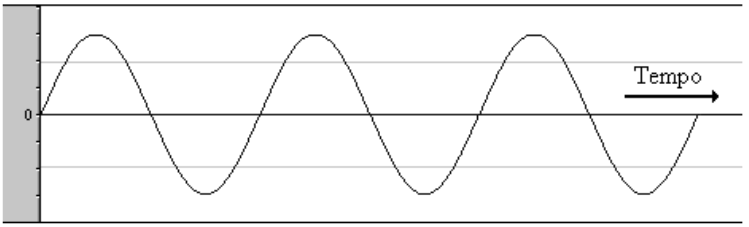
\includegraphics[scale=0.50]{figuras/ondaSenoidal.png}
   \\Fonte: \cite{miletto2004}
\end{figure}

Segundo \citeonline{miletto2004} e \citeonline{ferreira2015}, os cinco elementos básicos do som são:
\begin{enumerate}
\item \textit{Altura tonal}: É a “altura” de um som, ou seja, se é alto ou baixo, agudo ou grave. A repetição de uma onda periódica é chamada de ciclo. O número de ciclos dentro do intervalo de um segundo é chamado freqüência, medida em hertz (Hz), que é, então, a recíproca do período. Quanto maior o valor em hertz, mais agudo é o som. Dobrando a freqüência de um som, este é elevado em uma oitava. Então, é possível dizer que a freqüência e a altura tonal estão relacionadas logaritmicamente.

\item \textit{Volume}: A mudança no volume de um som pode ser vista como uma diferença na altura das ondas. A altura de uma onda chama-se “amplitude”. Quanto maior a amplitude, mais forte é o som. Portanto, o volume ou intensidade de um som é determinado pela amplitude.

\item \textit{Timbre}: É o que diferencia dois sons de mesma frequência. De um modo geral, formas de ondas arredondadas produzem um timbre mais suave, enquanto que as formas de ondas ponteagudas dão um timbre mais penetrante e estridente.

A Figura \ref{fig:ondaTimbre} mostra três formas de onda básicas, seus timbres característicos e os instrumentos que se assemelham a cada caso.

\begin{figure}[!htb]
   \centering
   \caption{Formas de onda simples e seus timbres}\label{fig:ondaTimbre} 
   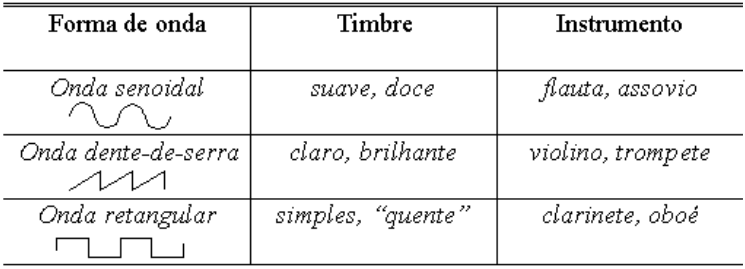
\includegraphics[scale=0.50]{figuras/ondaTimbre.png}
   \\Fonte: \cite{miletto2004}
\end{figure}

\item \textit{Envolvente da Onda}: É a variação da altura tonal, do volume e do timbre em um transcurso de tempo que vai desde o começo do som até um ponto do tempo onde ele desaparece completamente. Estas mudanças no tempo são o que determina o timbre característico de um objeto, além do seu espectro harmônico.

\item \textit{Duração}: A duração é responsável pelo tempo de emissão de um determinado som. Alguns sons possuem maior ressonância que outros, como um tambor que continua soando por um período de tempo curto, ou os sinos que soam por períodos maiores.
\end{enumerate}

Os sons com vibrações regulares - que são os harmônicos e a fundamental \footnote{Por definição, o primeiro harmônico corresponde à freqüência fundamental, o segundo harmônico ao primeiro harmônico e assim por diante \cite{muller2007}.} - são considerados sons musicais, enquanto os sons causados por vibrações irregulares - que não são harmônicos - cuja altura tonal não pode, portanto, ser medida, são chamados sons não-musicais. A maioria dos sons usados na música são, por pressuposto, sons musicais.

Á partir desses elementos, segundo \citeonline{ferreira2015}, temos a composição das propriedades da música, que são:

\begin{enumerate}
    \item \textit{Harmonia}: Pode ser definida como sendo o agrupamento sonoro. As combinações das notas tocadas simultaneamente de forma coordenada que compõem a harmonia.
    
    \item \textit{Melodia}: É a característica com maior destaque de uma música. Define-se como sendo uma sequência sonora tocada em intervalos irregulares.
    
    \item \textit{Ritmo}: Definido como a sequência de pulsações que se alternam entre sons e silêncios ao longo de um espaço de tempo.
\end{enumerate}

É possível ter uma melhor visualização da relação entre os elementos básicos do som e as propriedades da música na Figura \ref{fig:elementosMusica}.

\begin{figure}[!htb]
   \centering
   \caption{Relação entre elementos do som e da música}\label{fig:elementosMusica} 
   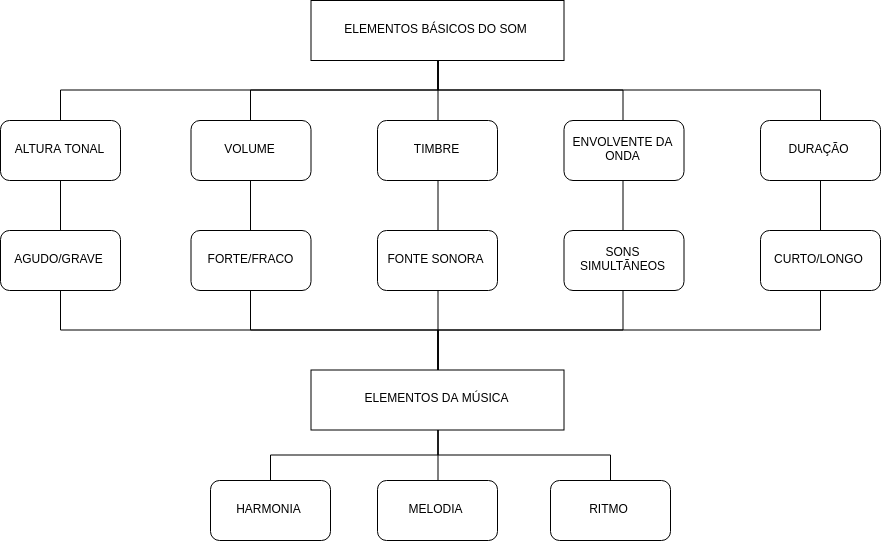
\includegraphics[scale=0.50]{figuras/elementosMusica.png}
   \\Fonte: \cite{ferreira2015}, adaptado pela autora
\end{figure}

%REPRESENTAÇÃO DO AUDIO DIGITAL%
\section{Representação do Áudio Digital} \label{sec:formatos}

Como comentado anteriormente, o som é a variação da pressão do ar. Sendo assim, a forma de produzir um determinado som depende da maneira como a pressão do ar varia. Para \citeonline{miletto2004}, o processo de representar numericamente o som é chamado de \textit{digitalização}, ou seja, é representar uma onda sonora (áudio analógico) em código binário (áudio digital). 

A digitalização das formas de onda consiste em três etapas realizadas por um circuito chamado \textit{conversor analógico/digital} (A/D) \cite{paulozuben2004}: \textit{amostragem}, \textit{quantização} e \textit{codificação}. Na primeira etapa, a forma de onda é lida ou amostrada em curtos intervalos de tempo uniformes (\textit{samples}). Na segunda etapa, o valor da forma de onda em cada ponto amostrado é restrito ou quantificado para um conjunto discreto de valores. Por fim, na terceira etapa é feita a codificação, traduzindo os valores para código binário. É uma transformação com perdas, ou seja, se perde informação neste processo (ver Figura \ref{fig:ondaAnalog}). Para podermos ouvir as informações transformadas em linguagem digital pelo conversor A/D é preciso realizar o processo inverso utilizando um \textit{conversor digital/analógico} (D/A) \cite{paulozuben2004}.

\begin{figure}[!htb]
   \centering
   \caption{Forma de onda analógica (curva preta) e representação digitalizada (as amostras digitalizadas são indicados pelas caixas cinzentas). Neste exemplo, a forma de onda é amostrada em 24 pontos e a quantização dos valores emprega um esquema de codificação de 4 bits (16 valores possíveis)}\label{fig:ondaAnalog} 
   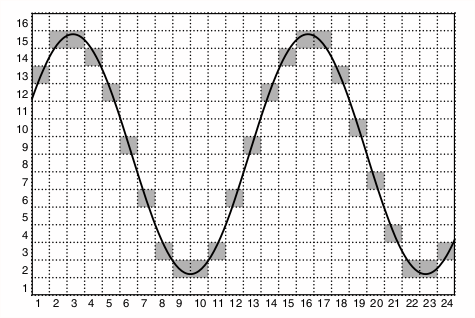
\includegraphics[scale=0.8]{figuras/ondaAnalog.png}
   \\Fonte: \cite{muller2007}
\end{figure}

Inicialmente, armazenar dados de áudio em formato analógico discretizado consome muito espaço \cite{juliana2004} e, como solução, foi adotada a codificação MIDI (\textit{Musical Instrument Digital Interface}). Essa codificação é uma representação numérica do som, sendo usada atualmente como o formato de intercâmbio de música digital simbólico mais comum para possibilitar a transferência de informações entre instrumentos musicais e computadores \cite{muller2007}. O tamanho desses arquivos tende a ser bem reduzido, já que a codificação de eventos musicais pode ser bem compacta.

Embora isso seja satisfatório em algumas situações, arquivos MIDI (extensão .mid ou .smf) basicamente codificam apenas instruções referentes a notas e durações e não a informação sonora propriamente dita \cite{fernando&kon1998}. Ou seja, seu código é composto por instruções para um sintetizador correspondente a eventos musicais como soar uma nota, silenciar uma nota, mudar o andamento ou o tom da música, etc. O sintetizador, por sua vez, interpreta este código e o executa, podendo usar vários timbres de instrumentos simultaneamente \cite{miletto2004}. Por isso, o resultado sonoro é totalmente dependente da qualidade e das possibilidades oferecidas por esse aparelho \cite{fernando&kon1998}.

Com o mesmo objetivo, os formatos \textit{Wave}, da Microsoft (extensão .wav), e \textit{AIFF}, da Apple (extensão .aiff ou .aif) são do tipo áudio digitalizado sem compressão. Baseiam-se na codificação PCM (\textit{Pulse Code Modulation}), onde a própria onda sonora é representada como uma sucessão de números correspondentes às amplitudes do sinal medidas a uma freqüência constante. Ou seja, armazenam dados de um processo de digitalização simples. A diferença para o formato MIDI é que esse tipo de codificação origina um grande volume de dados e exige muito espaço para armazenamento. Sua única vantagem é a reprodução fiel do áudio se o arquivo for gravado com qualidade de CD \cite{miletto2004}.

Outro recurso é a compressão de dados, que é feita através de programas ou \textit{hardware} específicos que compactam os arquivos de áudio, reduzindo o seu tamanho antes de serem enviados. Ao chegar ao seu destino, esses arquivos são descompactados e, em seguida, tocados. Entretanto, compressão, nesse contexto, é sinônimo de perda de qualidade: quanto maior a compressão, maior também a quantidade de informação que se perde \cite{fernando&kon1998}. Apesar disso, certos padrões de compressão já permitem a transmissão de arquivos de áudio de boa qualidade em tempo real, o que resulta na existência de uma quantidade equivalente de formatos de arquivo para a compressão do som digitalizado \cite{miletto2004}.

Segundo \citeonline{miletto2004}, os formatos de arquivo mais utilizados para a compressão de som são:

\begin{itemize}
    \item MPEG Layer 3 (extensão .mp3);
    \item Advanced Audio Coding (extensão .aac);
    \item Windows Media Audio, da Microsoft (extensão .wma);
    \item Real Audio, da RealNetworks (extensão .ra);
    \item Sun Audio, da Sun (extensão .au).
\end{itemize}

Em paralelo, quando o áudio foi do analógico para o digital, tornou-se possível codificar arquivos de áudio com mais informação do que apenas o nome do arquivo, utilizando-se dos chamados \textit{metadados}.

Metadados podem ser usados para nomear, descrever, catalogar e indicar os direitos de autor de um arquivo de áudio digital. Como diferentes formatos de áudio digitais foram desenvolvidos, foi acordado que um local padronizado e específico seria reservado dentro dos arquivos digitais, onde estas informações pudessem ser armazenadas \cite{pachecolopes2014}. Existem padrões diferentes de metadados para finalidades distintas de informações. Para o áudio digital, o padrão mais utilizado é o de \textit{tags} ID3\footnote{Embora referido como um padrão, o termo se aplica apenas no sentido de palavra, já que nenhum organismo de normalização foi envolvido na sua criação, e nenhuma dessas organizações lhe deu esse estatuto de aprovação formal \cite{pachecolopes2014}.} (abreviação de \textit{IDentify a MP3}). 

O ID3 começou a ser idealizado a partir de 1996 por Eric Kemp\footnote{http://id3.org/}. Em sua primeira versão, o ID3 limitava-se apenas a 128 KB\abreviatura{KB}{\textit{Kilobyte}} de informação, e essas informações também eram limitadas quanto ao número de caracteres. Já na segunda versão, idealizada a partir de 1998, o padrão tornou-se mais completo, permitindo que mais informações pudessem ser adicionadas, já que o limite passou a ser de 256 MB \abreviatura{MB}{\textit{Megabyte}} \cite{ferreira2015}.

Na Tabela \ref{tab:diferencasId3} é possível verificar as diferenças com relação aos metadados considerados pelas versões do ID3.

\begin{table}[ht]
    \centering
    \caption{Diferenças entre as versões ID3}
    \begin{tabular}{p{4cm}|p{4cm}}
    \hline
        ID3v1 & ID3v2 \\
    \hline
        128 B & 256 MB \\
    \hline
        Título & Título \\
    \hline
        Artista & Artista \\
    \hline
        Álbum & Álbum \\
    \hline
        Ano & Ano \\
    \hline
        Comentário & Comentário \\
    \hline
        Gênero & Gênero \\
    \hline
         & Compositores \\
    \hline
         & Letra da música \\
    \hline
         & Capa do álbum \\
    \hline
    \end{tabular}
    \label{tab:diferencasId3}
    \\Fonte: \cite{ferreira2015}, adaptado pela autora
\end{table}

Segundo \citeonline{pachecolopes2014}, metadados podem ser armazenados de duas formas:

\begin{itemize}
    \item Interno (ou incorporado): os metadados são transportados como parte do arquivo de áudio digital;
    \item Externo: os metadados podem ser unidos com o conteúdo quando a informação é transferida ou referenciada.
\end{itemize}

Um Banco de Dados(BD) \abreviatura{BD}{Banco de Dados} normalmente armazena os metadados externamente, mas pode ser projetado para suportar abordagens para o armazenamento interno de metadados. Cada qual apresenta vantagens e desvantagens, como pode ser visto na Tabela \ref{tab:diferencasArmazenamentoMetadados}.

\begin{table}[ht]
    \centering
    \caption{Diferenças entre as formas de armazenamento de metadados}
    \begin{tabular}{p{5cm}|p{5cm}}
    \hline
        Armazenamento Interno & Armazenamento Externo \\
    \hline
        Não permite a gestão de todos os metadados em um só lugar & Procura e gestão mais eficiente dos metadados \\
    \hline
        Cria redundância impedindo a normalização & Evita redundância através da normalização \\
    \hline
        Os metadados estão sempre disponíveis e podem ser manipulados no local & Os arquivos sozinhos não transportam os metadados \\
    \hline
    \end{tabular}
    \label{tab:diferencasArmazenamentoMetadados}
    \\Fonte: Elaborado pela autora
\end{table}

Existem diversos \textit{softwares} que editam as \textit{tags} ID3, porém, na maioria das vezes esses \textit{softwares} disponíveis não permitem a edição completa dos dados de descrição do áudio.

Desta forma, podemos afirmar que um arquivo de áudio digital é composto por metadados e som digitalizado, sendo assim, um dado musical.

%INFORMAÇÃO MUSICAL%
\section{Informação Musical} \label{sec:informacao-musical}
Para \citeonline{setzer2001}, dado é uma sequencia de números, portanto, um texto, fotos, figuras, sons gravados e animação são dados, pois todos podem ser amostrados, quantificados e codificados. Um dado é necessariamente uma entidade matemática e, desta forma, é puramente sintático. Isto significa que os dados podem ser totalmente descritos através de representações formais, estruturais e obviamente ser armazenados em um computador e processados por ele.

O dado é a representação física de um evento no tempo e espaço que não agrega fundamento, não sendo possível entender o que ele representa ou para que ele existe, se somente for disponibilizado para alguém ou para o tempo e espaço, por alguém ou por um evento.
Entretanto, ao incluir um “significado” no dado e gerar sentido para quem o ouve e ficando claro ou não a que se refere, é gerada a informação \cite{rafael2013}.

O autor \citeonline{setzer2001} expõe que a informação é uma abstração informal (isto é, não pode ser formalizada através de uma teoria lógica ou matemática) que está na mente de alguém, representando algo significativo para essa pessoa. A frase “Paris é uma cidade fascinante” é um exemplo de informação desde que seja lida ou ouvida por alguém, desde que "Paris"\ signifique para essa pessoa a capital da França (supondo-se que o autor da frase queria se referir a essa cidade) e "fascinante"\ tenha a qualidade usual e intuitiva associada com essa palavra.

A informação pode ser armazenada em um computador, ou melhor, a sua representação em forma de dados e não a informação propriamente dita. Essa representação pode ser transformada pela máquina, como na formatação de um texto, mas não pode mudar o significado, já que ela depende de uma pessoa que possui a informação. Os dados são sempre incorporados por alguém como informação, porque os seres humanos buscam constantemente por significação e entendimento.

A partir daí, a autora \citeonline{barros2012} expõe que um dado musical é resultado de um processo de significação social. Assim, a música é uma expressão humana construída socialmente e objetivada por meio de sua comunicação oral, registro sonoro ou representação gráfica.

Para \citeonline{almeida2007}, a obra musical é efêmera e abstrata, pois só se concretiza no momento de cada interpretação, na execução da música. 

\citeonline{berger&luckmann2014} afirmam que:

\begin{citacao}
A expressividade humana é capaz de objetivações, isto é, manifesta-se em produtos da atividade humana que estão ao dispor, tanto dos produtores quanto dos outros homens, como elementos que são de um mundo comum \cite{berger&luckmann2014}.
\end{citacao}

Para \citeonline{angeles2010,pinheiro&loureito1995}, a informação é o que se acrescenta a uma representação. Segundo os autores, recebemos informação se o que conhecemos é alterado. Informação é o que logicamente justifica alteração ou reforço de uma representação, ou de um estado de coisas. As representações podem ser explícitas (como em um mapa ou em uma proposição), ou podem estar implícitas no estado de atividade dirigida do receptor.

A informação musical apresenta determinadas especificidades de comportamento na sua produção, objetivação e uso, pois a manifestação da música apresenta-se carregada de características próprias. \citeonline{michels1992} explica que a música contém dois elementos: o \textit{material acústico} e a \textit{ideia intelectual}, sendo que tais elementos não se encontram justapostos, mas sim se combinam para formar uma imagem unitária. Portanto, a compreensão completa da música está diretamente ligada com o reconhecimento do contexto histórico e social de sua origem, com a interpretação pessoal e individual do ouvinte, e com os aspectos sonoros que a constituem. Dessa forma, a música tem diferentes significações para cada indivíduo.

\citeonline{lima&santini2006} afirmam que:

\begin{citacao}
A música é um produto social e simbólico de grande importância nas diferentes formações culturais, principalmente se considerarmos a sua capacidade de criar vínculos afetivos e cognitivos entre as pessoas \cite{lima&santini2006}.
\end{citacao}

A compreensão da música como informação é ainda bastante recente. O estudo mais significativo e considerado, dentro da literatura especializada, como pioneiro na conceituação e estudo da música como fonte de informação é o de Alexander McLane. Em 1996, o autor publicou em um capítulo do \textit{ARIST} (\textit{Annual Review of Information Science and Technology}) o artigo intitulado \textit{Music as Information}, onde formaliza a música como informação.

%ARMAZENAMENTO DA INFORMAÇÃO MUSICAL%
\section{Armazenamento da Informação Musical} \label{sec:armazenamento}

Até o surgimento dos inventos tecnológicos, a música era um meio de comunicação exclusivamente presencial. Apesar das formas de registros, a exemplo das partituras, possibilitarem a execução de uma obra em diferentes momentos e lugares, a reprodução do que ali estava representando nunca seria a mesma. Com o decorrer do tempo,  as técnicas e invenções aplicadas ao processo de gravação do som foram surgindo e se aperfeiçoando, resultando em aparelhos reprodutores e suportes cada vez mais versáteis e manipuláveis \cite{daquino2012}. Especialmente após o desenvolvimento das coleções em rede na \textit{Web}, com formatos de arquivos compactados e custos decrescentes de armazenamento de arquivos na forma digital, a música se tornou um objeto de consumo universal e extremamente acessível \cite{gomes2015}.

Os dispositivos de armazenamento musical são divididos em dois grandes grupos: \textit{analógicos} e \textit{digitais} \cite{andrade&crispim2008}. Os analógicos são antecessores dos digitais e foram o meio tecnológico dominante em boa parte do século XX \cite{paulozuben2004}. O primeiro invento significativo foi o fonógrafo, patenteado por Thomas Edison em 1877. Dez anos mais tarde, em 1887, surgiu o gramofone, tendo uma capacidade maior de armazenamento e reprodução das músicas \cite{marchi2005}. 

Dentre as invenções mais importantes para o armazenamento e a reprodução sonora analógica está o disco de vinil, lançado em 1948, comumente conhecido como LP\abreviatura{LP}{\textit{long-play}}. Era um disco com rotação por minuto mais demorada, o que permitia aumentar a capacidade de armazenamento da informação na superficie do vinil. Em seguida, entre as décadas de 60 e 70, com a evolução dos cartuchos 8-track (pioneiros em armazenar dados musicais em fitas magnéticas), o lançamento da fita cassete ou \textit{compact cassette} \cite{marchi2005} era basicamente, dois carretéis, a fita magnética e todo o mecanismo de movimento da fita, alojados em uma caixa plástica \cite{andrade&crispim2008}.

No armazenamento analógico, as formas de onda dos sinais elétricos emitidos do aparelho eram registradas similarmente, isto é, de maneira análoga, pelas partículas magnéticas encontradas na fita. No momento da reprodução, os sinais magnéticos impressos na fita são interpretados analogamente como diferenças de voltagem, isto é, sinais elétricos. Como o nível do sinal elétrico era muito baixo, utilizava-se um amplificador para que a variação de voltagem seja suficiente para mover os cones dos alto-falantes. Dizemos que esse processo é uma gravação analógica, pois a forma de onda do sinal gravado é análoga à forma de onda do sinal original captado \cite{paulozuben2004}.

Porém, a partir da década de 80, com a intensificação do uso de \textit{hardwares} e \textit{softwares}, surge um dos primeiros meios de armazenamento digital: o CD (\textit{Compact-Disc}). Ele acabou por se tornar um dos meios de armazenamento de dados musicais mais populares das décadas seguintes. Além de quebrar paradigmas na época, o CD foi inspiração para o desenvolvimento de outros meios de armazenamento como os DVDs\abreviatura{DVD}{\textit{Digital Versatile Disc}} e os discos de Blu-ray \cite{marchi2005}.

Entretanto, surgiu a necessidade de disponibilizar informações nos dispositivos de armazenamento. Na era analógica, esses recursos estavam associados à capa e/ou contracapa. Todavia, com a mudança do paradigma para digital, necessitou-se que essas informações pudessem ser disponibilizadas digitalmente, porém, o CD de áudio não inclui em sua estrutura, por exemplo, o nome do disco ou o nome de suas faixas. Sendo assim, surgiram as bases de dados de CDs, que visam prover informações dos mesmos quando esses são utilizados por sistemas de mídia modernos \cite{andrade&crispim2008}.

Com o surgimento dos arquivos digitais de áudio, as músicas se desvincularam do suporte físico (CD) e passaram a ser vistas isoladamente. Esses tipos de arquivos requerem um espaço consideravel para seu armazenamento (chegando a ocupar dezenas de megabytes em disco), o que propiciou o surgimento de um formato mais compacto: O MP3 (\textit{Moving Picture Experts Group-1 Layer 3}).

O grande desenvolvimento tecnológico das redes de compartilhamento de arquivos contribuiram para uma maior aceitação de formato de áudio MP3 \cite{andrade&crispim2008}, por ser facilmente transportado em qualquer bolso ou mochila e pela sua longa vida útil, além do aumento gradativo de armazenamento com o passar dos anos \cite{marchi2005}. Sua invenção, propiciou a popularização de eletrônicos com portas USB e o surgimento de cartões de memória \textit{microSD}, prometendo maior capacidade, durabilidade e clareza sonora \cite{marchi2005}.

Com a Internet, a música ultrapassa os limites físicos da mídia - mergulhando no universo digital - e passa a circular livremente pela rede mundial de computadores através do \textit{streaming}, que tomou forma no final da década de 80 e começou a se desenvolver na década de 90, com a evolução dos SGBDs \abreviatura{SGBD}{Sistema de Gerenciamento de Banco de Dados} (\textit{Sistemas de Gerenciamento de Banco de Dados}) e o surgimento dos BDOOs (\textit{Bancos de Dados Orientado a Objetos}) \cite{junior&segundo2008}, que possibilitaram o armazenamento de multimidias, assim como a popularização de aplicativos móveis, conhecidos normalmente por \textit{apps}, que oferecem mais de 30 milhões de músicas a seus usuários, como por exemplo, "Spotify"\footnote{https://www.spotify.com/br/} e "Deezer"\footnote{https://www.deezer.com/br/}.

Ainda, para uma eficiente recuperação de informação é preciso que o conjunto dos arquivos musicais estejam representados de forma adequada, contemplando as possíveis informações que o usuário busca \cite{ferreira2015}.

%RECUPERAÇÃO DA INFORMAÇÃO MUSICAL%
\section{Recuperação da Informação Musical} \label{sec:recuperacao}

A área de pesquisa denominada \textit{Music Information Retrieval} (MIR - \textit{Music Information Retrieval}) ou Recuperação da Informação Musical (RIM), tradução literal incorporada pela corrente da área no Brasil, é definida, de acordo com \citeonline{futrelle&downie2002}, como:

\begin{citacao}
[...] uma agenda de pesquisa que, de forma geral, pretende desenvolver formas de gestão de coleções de obras musicais para preservação, busca, acesso e outros usos \cite{futrelle&downie2002}.
\end{citacao}

A agenda de pesquisas sobre a MIR intensificou sua produção recentemente com a explosão do interesse em coleções em rede que contenham obras musicais na forma digital, possibilitadas pelo desenvolvimento das citadas técnicas de compressão de áudio. Os pesquisadores de MIR observam que a motivação maior para essa área de pesquisa é o grande volume de música digital disponível na Internet que, quanto mais cresce, menos possibilita sua recuperação eficiente, visto que estão apenas disponíveis em grande quantidade, mas sem o tratamento adequado \cite{gomes2015}.

A área de MIR conta com profissionais das mais diversas áreas inclusas na questão do tratamento e recuperação da informação musical como apresentado na Tabela \ref{tab:comunidadeMIR}, traduzida por \citeonline{santini&souza2007}.

\begin{table}[ht]
    \centering
    \caption{Comunidades de MIR}
    \begin{tabular}{p{4cm}|p{4cm}|p{4cm}}
    \hline
        Comunidade & Tipo(s) de instituição & Área de pesquisa \\
    \hline
        Ciência da Computação, Recuperação da Informação & Acadêmica, Comercial & Representação, Indexação, Recuperação, Aprendizado de máquina, Design de interface de uso \\
    \hline
        Engenharia de áudio, Processamento de sinais digitais & Acadêmica, Comercial & Compressão, detecção de critério, Localização de tom, Aprendizado de máquina, Classificação, Análise musical \\
    \hline
        Musicologia, Teoria Musical & Acadêmica & Representação, Análise musical \\
    \hline
        Ciência da Informação, Biblioteconomia & Bibliotecas, Acadêmica & Representação, Metadados, Estudos de usuário, Classificação, Direitos de propriedade intelectual, Design de interface de uso \\
    \hline
        Ciência Cognitiva, Psicologia, Filosofia & Acadêmica & Representação, Percepção, Estudos de usuário, Ontologia \\
    \hline
        Direito & Governamental, Profissionais da lei, Acadêmica & Direitos de propriedade intelectual \\
    \hline
    \end{tabular}
    \label{tab:comunidadeMIR}
    \\Fonte: \apud{santini&souza2007}{futrelle&downie2002}
\end{table}

A origem de MIR não apresenta uma ação interdisciplinar, o que prejudica todo o seu processo de comunicação científica. Como pontua \citeonline{santini&souza2007}:

\begin{citacao}
(...) não há uma sociedade (inter)disciplinar de MIR; um periódico ou livro-texto fundador onde pessoas interessadas podem adquirir as bases teóricas e práticas de MIR. Com exceção de alguns pequenos encontros interdisciplinares, muitos pesquisadores estão apresentando seus resultados para membros das suas próprias disciplinas. A literatura de MIR é difícil de ser localizada, lida e estudada, o que dificulta construir e sustentar uma área de pesquisa respeitável e próspera \cite{santini&souza2007}.
\end{citacao}

A escassa produção científica a respeito do tema e as características impostas pelas músicas acarretam certas dificuldades para sua representação.

Como elucidado no final da subseção 2.1 desta seção, o ponto de partida para os estudos sobre a música como fonte de informação e tratamento, representação e recuperação foi dado em 1996 por Alexander McLane. Neste mesmo período já era possível identificar o desenvolvimento de tecnologias de compressão de arquivos digitais de música para transmissão na Internet e a popularização da Internet no mundo \cite{santini&souza2007}.

Em seu estudo, McLane direciona sua discussão para os grandes problemas relacionados à representação de documentos de música e à recuperação destes documentos. Ele analisa aspectos significantes da música – sua notação e seu som –, e propõe algumas ideias para sistemas de recuperação de música e formaliza a música como informação segundo três visões: \textit{visão subjetiva}, \textit{visão objetiva} e \textit{visão interpretativa}. Segundo o autor, as necessidades dos vários tipos de análises musicais são tão diversas que é preferível considerar três “visões” sobre a representação da obra musical.

Em resumo adaptado, \citeonline{santini&souza2007} apresentam as principais características das visões estabelecidas por \citeonline{mclane1996}.

\begin{itemize}
    \item A visão \textit{subjetiva} da informação musical se faz por meio do uso do esquema de notação para representação da informação musical. A subjetividade se dá porque a escolha de elementos de notação geralmente representa uma obra em “contexto-dependente”. Sendo assim, a decisão da notação pode incluir ou excluir aspectos particulares da obra.
    \item A visão \textit{objetiva} está vinculada a audição e ao momento da execução musical. Um som gravado pode ser identificado como visão objetiva da obra musical. A sonoridade se caracteriza como objetiva por não se configurar como uma representação, mas como a obra em sua essência. O som musical uma vez gravado torna-se fixo e não está mais sujeito a variações editoriais e de performance. Segundo McLane, esta visão pode ser considerada a mais completa representação da música, ao passo em que inclui as facetas tom, tempo, harmonia, editorial e timbre.
    \item A visão \textit{interpretativa} é realizada através da análise de alguns aspectos da obra, englobando informações que não são diretamente dependentes do documento. Entram nessa categoria classificações e esquemas analíticos que elucidam características como o gênero musical e avaliações críticas.
\end{itemize}

De acordo com \citeonline{cruz2014}:

\begin{citacao}
Dentre as visões propostas por \citeonline{mclane1996}, a interpretativa possui uma característica interessante porque permite a independência formal do documento musical em relação ao suporte que o contém, assim como foi possível na informação textual \cite{cruz2014}.
\end{citacao}

Segundo \citeonline{mclane1996,santini&souza2007}, a representação da informação musical pode abranger as três visões apresentadas dependendo das necessidades de informação da comunidade usuária. De acordo com tradução das autoras, a conclusão de McLane seria a de que:

\begin{citacao}
Ambas as escolhas sobre a visão da representação da música e o grau de complementação da representação de uma obra depende da necessidade de informação do usuário. A recuperação de informação é um processo interativo que depende do conhecimento do usuário e do nível de complexidade da informação desejada. No caso da necessidade da simples identificação de uma obra musical, onde a informação bibliográfica não é unicamente suficiente, pode-se limitar a uma visão subjetiva envolvendo um subconjunto relativamente pequeno de elementos notados de uma obra, frequentemente o tom inicial de uma frase melódica. A representação tonal pode ser de forma tal que provavelmente o usuário espera e está apto para formular a indagação usando a mesma terminologia, ou pelo menos uma que é traduzível na forma de representação \apud{santini&souza2007}{mclane1996}.
\end{citacao}

Sendo assim, percebe-se que a recuperação da informação da música depende tanto da complexidade e da forma como a informação é representada, como do nível de conhecimento prévio do usuário. Para \citeonline{santini&souza2007}: “Quanto menor o conhecimento do usuário, maior a necessidade de diferentes formas de representação. Cada visão da representação da música, demonstrada por McLane, não é suficientemente isolada para identificar uma obra.”.

Outro autor presente nos estudos relacionados à representação e recuperação de informação musical e um dos representantes da área de MIR é o professor J. Stephen Downie da Universidade de Illinois, nos Estados Unidos. Downie escreveu, em 2003, outro artigo tido como marco no estudo da informação musical, intitulado \textit{Music Information Retrieval} também em um capítulo do ARIST. No trabalho em questão, \citeonline{downie2003} examina a multidisciplinaridade da área de MIR, identifica e explica alguns problemas relacionados à questão da representação e recuperação da informação musical. Para isso, \citeonline{downie2003} resume a questão em quatro grandes desafios a serem enfrentados pelos pesquisadores da área:

\begin{citacao}
    \begin{enumerate}
        \item Considerar permanentemente as diferentes formas de representação da música, o que caracteriza o \textit{desafio multirepresentacional}. O copyright faz parte deste desafio.
        \item Cada época histórica e cada formação cultural criam modos próprios e singulares de se expressar através da música. A música transcende as fronteiras culturais e temporais. A ampla variedade de expressões musicais coloca em evidência o \textit{desafio multicultural}.
        \item Compreender e responder às diferentes formas de interação individual com a música e com os sistemas de MIR constitui o \textit{desafio multiexperimental}.
        \item Maximizar os benefícios de ter uma comunidade multidisciplinar de pesquisadores, enquanto minimiza a desvantagem inerente, representa o \textit{desafio multidisciplinar}.
    \end{enumerate} 
\end{citacao}

O desafio multirepresentacional é dividido em sete facetas a serem consideradas na descrição da música e que representam a estrutura musical \cite{downie2003}: tonal, temporal, harmônica, de timbre, editorial, textual e faceta bibliográfica, sendo as quatro primeiras relativas a aspectos sonoros da música com formas gráficas de representação em figuras rítmicas ou notações musicais, enquanto que as três últimas são representadas na forma gráfica e dizem respeito às informações de produção, intérprete, compositor, copyright, data de produção e outras \cite{barros2012}.

Apesar de completas, a interação dessas facetas resulta em um complexo tratamento da informação musical, visto que cada faceta citada possui, por si só, uma complexidade inerente e sofre um tipo de representação enquanto produto. As autoras \citeonline{santini&souza2007} resumem a problemática multirepresentacional da seguinte forma:

\begin{citacao}
    A complexa interação entre as facetas da música - tonal, temporal, harmônica, de timbre, editorial, textual e bibliográfica – evidencia um dos principais problemas de MIR: o desafio multirepresentacional. A escolha da representação da música – se baseada em símbolos, áudio ou ambos – adiciona-se a diversas questões: como, por exemplo, cada escolha determina a tecnologia, a organização, a recuperação e a interface entre requisitos e capacidades dos sistemas \cite{santini&souza2007}.
\end{citacao}

Sendo assim, apesar de possuir as facetas estabelecidas por \cite{downie2003}, a estrutura da música incorpora elementos extras que nos permitem defini-la como um objeto informacional mais complexo. Para \citeonline{cruz2014} a estrutura musical:

\begin{citacao}
    [...] incorpora elementos adicionais que permitem defini-la como um objeto informacional musical mais amplo, dotado de conteúdo – atributos internos e metadados descritivos – e, de contexto – associações com outros objetos musicais e não musicais, e com situações ou eventos em que este objeto musical está inserido \cite{cruz2014}.
\end{citacao}

O segundo desafio (multicultural) nasce da condição inerente à música de ser uma objetivação de algo extremamente subjetivo: a \textit{expressão humana}. Sendo assim, sofre a interferência de uma grande variedade de fatores, da cultura vigente no momento da produção musical e da localização geográfica desta produção.

O desafio multiexperimental diz respeito à percepção da música como experiência individual ou coletiva capaz de causar diferentes reações em diferentes momentos e situações, de cada mente e humor individual. Neste caso, ouvir uma música gravada funciona como “ajudar a memória” que traz a tona experiências prazerosas ou dolorosas relacionadas a uma música em especial \cite{downie2003,santini&souza2007}. As variações de pessoa para pessoa na forma de apropriação, apreciação e nos tipos de experiências emocionais que a música evoca demonstram de maneira pragmática o desafio multiexperimental.

O quarto e último desafio estabelecido por \citeonline{downie2003} é o desafio multidisciplinar. Como citado anteriormente, a diversidade intelectual da comunidade de pesquisadores de MIR é, ao mesmo tempo, uma vantagem e uma adversidade. A heterogeneidade das visões de mundo das disciplinas apresenta um problema particular. Cada disciplina traz suas crenças, práticas, questões de pesquisa e paradigmas de avaliação \cite{downie2003}. De acordo com \citeonline{futrelle&downie2002}, não há uma aceitação comum dos objetivos, técnicas e resultados obtidos nas pesquisas referentes à informação musical.

Percebe-se, portanto, que, se por um lado, a ação multidisciplinar dos pesquisadores envolvidos com o tema possibilita o surgimento de diversos avanços tecnológicos e que a cada dia são divulgadas novas soluções para o tratamento de conteúdos musicais, com algoritmos mais sofisticados, novas formas de indexação de músicas, novos tipos de interfaces de áudio e novas formas de representação musical, em contrapartida, é notável a dificuldade de comunicação entre esses resultados. Nota-se ainda a dificuldade de identificação desses conteúdos musicais, porque a música é complexa e possui um leque de propriedades que possibilitam abordagens, às vezes, contraditórias \cite{cruz2014}.

A análise da informação musical para sua representação apresenta complexidades, pois exige diferentes técnicas de extração de informações para distintas formas de apresentação \cite{downie2003}.

%MÉTODOS E ALGORITMOS PARA RECUPERAÇÃO DA INFORMAÇÃO MUSICAL%
\subsection{Métodos e Algoritmos para Recuperação da Informação Musical} \label{subsec:metodos-algoritmos-recuperacao}

Um dado musical geralmente é representado por um conjunto de características extraídas do conteúdo da música. Isto porque dados musicais são basicamente arranjos multidimensionais de valores derivados de vários sensores, que é uma representação limitada para definir a semântica do dado. Neste sentido, dados complexos raramente são comparados diretamente. Em vez disso, o conteúdo do dado (ou uma faceta do conteúdo) é analisado por meio de algoritmos especializados de análise, extraindo um conjunto de características que descrevem numericamente o dado \cite{kaster2012}. Desta forma, as aplicações que lidam com dados complexos, como dados musicais, requerem a realização de consultas por similaridade, ou seja, consultas que realizam busca por objetos da base que sejam similares a um objeto de consulta, de acordo com uma certa medida de similaridade \cite{barioni2006}.

A Sociedade Internacional de Recuperação da Informação Musical (ISMIR\footnote{https://transactions.ismir.net/}\abreviatura{ISMIR}{\textit{International Society for Music Information Retrieval}}, na sigla em inglês) abriga, durante sua conferência anual, o MIREX\footnote{http://www.music-ir.org/mirex/wiki/MIREX\_HOME}\abreviatura{MIREX}{\textit{Music Information Retrieval Evaluation eXchange}}, com o objetivo de estabelecer métodos para a avaliação e comparação das aplicações atuais de recuperação musical. Nesta espécie de competição, pesquisadores inscrevem algoritmos que realizam diferentes tarefas da área de recuperação da informação musical, como classificação automática de gênero musical, identificação automática da pulsação, extração de melodia a partir de arquivos áudio, entre outros.

\begin{figure}[!htb]
   \centering
   \caption{Representação do modelo de recuperação de informação musical} 
   \label{fig:modeloRecInfo} 
   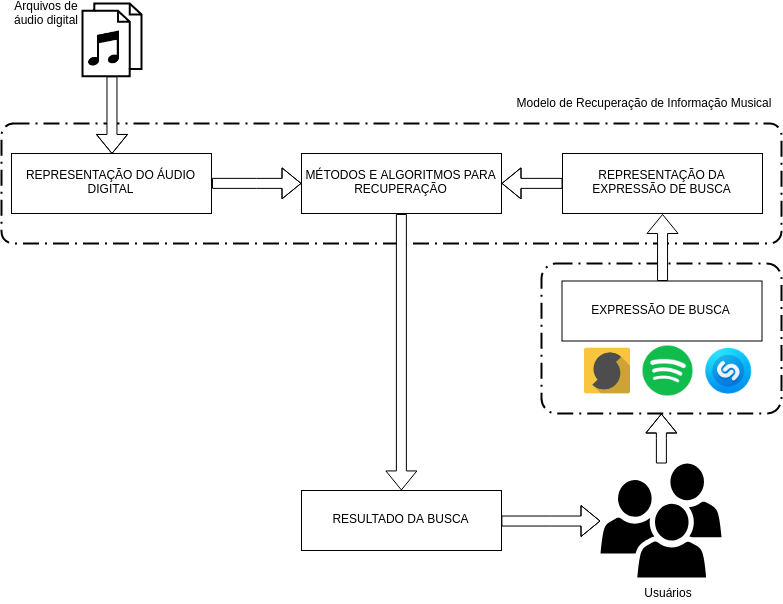
\includegraphics[scale=0.47]{figuras/modeloRecInfo.png}
   \\Fonte: \cite{ferreira2015}, adaptado pela autora
\end{figure}

Um sistema de recuperação de informação musical atua, portanto, como um ambiente mediador da comunicação entre as necessidades informacionais dos usuários e o conjunto de arquivos de áudio. Na Figura \ref{fig:modeloRecInfo} é possível compreender melhor o processo de recuperação de informação. Dadas as características de um sinal de áudio, pode-se definir métricas de similaridade para comparar músicas. Embora exista uma grande variedade de funções de distância disponível na literatura, não existe um método que determine, de um modo geral, qual deve ser a melhor função de distância a ser utilizada em cada caso. A escolha ou definição de uma função de distância é uma tarefa que depende muito da análise das características específicas do domínio dos dados a serem manipulados \cite{barioni2006}.

O foco deste trabalho não é aprofundar o conhecimento nos métodos e algoritmos utilizados para recuperação da informação musical. Assim sendo, os principais métodos e algoritmos disponíveis na literatura são descritos aqui de forma breve.

%AUDIO FINGERPRINT%
\subsubsection{Audio Fingerprint} \label{subsubsec:audioFingerprint}
\textit{Audio Fingerprint} é como uma assinatura única de uma música, contendo um sumário de suas características que resume uma gravação de áudio. \citeonline{cano2005} que definem que uma \textit{fingerprint} de áudio é um resumo digital, que pode ser utilizado para identificar uma amostra ou localizar rapidamente itens semelhantes em uma base de dados de áudio, independente do nível de compressão, distorção ou interferência no canal de transmissão.

Esse sistema pode ser separado em dois processos fundamentais: extração do \textit{fingerprint} (\textit{frontend}) e o algoritmo de comparação (\textit{match}). Estes, por sua vez, são divididos em até oito etapas, conforme mostrado na Figura \ref{fig:etapasFinger}.

\begin{figure}[!htb]
   \centering
   \caption{Diagrama de identificação de áudio} \label{fig:etapasFinger} 
   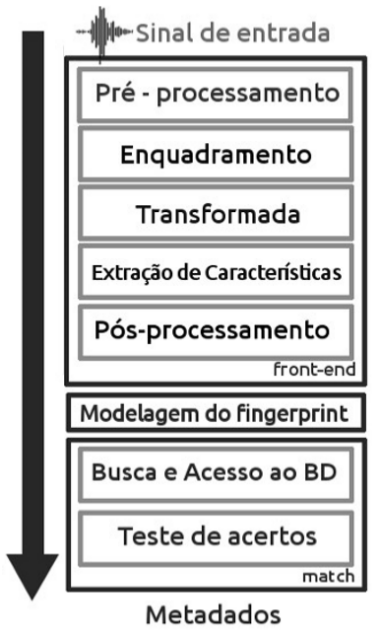
\includegraphics[scale=0.47]{figuras/etapasFinger.png}
   \\Fonte: \cite{carreira2015}
\end{figure}

No processo de \textit{frontend} há uma sequência de métodos relevantes até a criação de fato do \textit{fingerprint}. Segundo \citeonline{cano2005}, o primeiro passo é o pré-processamento, onde o som é digitalizado (se necessário) e convertido em um formato genérico, por exemplo, para o formato de 16 bits PCM\footnote{\textit{Pulse Code Modulation}: método usado para representação digital de sinais analógicos.}.

O enquadramento adapta a amostragem convertida para o que será utilizado e \citeonline{cano2005} definem que:

\begin{citacao}
[...]o sinal é dividido em quadros de um tamanho comparável à velocidade de variação dos eventos acústicos subjacentes. O número de quadros calculados por segundo é chamado de taxa de quadros. Uma função de janela cônica é aplicada a cada bloco para minimizar as descontinuidades no início e no final. A sobreposição deve ser aplicada para garantir robustez ao deslocamento (ou seja, quando os dados de entrada não estão perfeitamente alinhados com a gravação usada para gerar a \textit{fingerprint}) \cite{cano2005}.
\end{citacao}

Em seguida, precisa-se ter o áudio no domínio da frequência \cite{bunnell1996a}. Assim, transformações adicionais são aplicadas que convertem esses sinais em função da frequência, para que o algoritmo de reconhecimento possa realizar uma melhor classificação dentro das características desejadas \cite{santos2011}.

\citeonline{cano2005} citam algoritmos de Transformadas para facilitar a compressão eficiente, a remoção de ruídos e o processamento subsequente:

\begin{itemize}
    \item Transformada de Karhunen-Loève;
    \item Tranformada Rápida de Fourier;
    \item Transformada de Walsh-Hadamard;
    \item \textit{Modulated Complex Lapped Transform (MCLT)};
    \item Transformada Wavelet.
\end{itemize}

\citeonline{santos2011} cita um algoritmo prático conhecido como o \textit{espectro do produto harmônico}, ou HPS. Esse algoritmo parte do princípio que o espectro da janela de um sinal de áudio é formado por picos de energia situados na fundamental e na série harmônica da nota. O processo seguido pelo algoritmo é ilustrado na Figura \ref{fig:hps} e consiste em multiplicar o espectro do sinal, obtido a partir do algoritmo da Trasformada, por versões comprimidas do próprio espectro. A compressão é realizada reduzindo a amostragem do espectro original por fatores inteiros.

\begin{figure}[!htb]
   \centering
   \caption{Processo da Técnica HPS}\label{fig:hps} 
   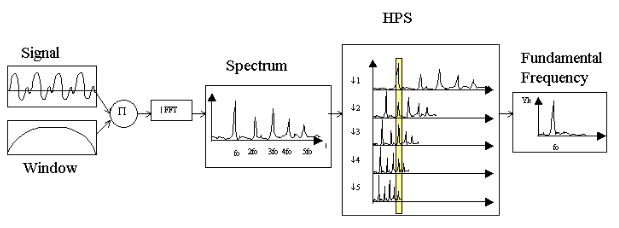
\includegraphics[scale=0.62]{figuras/hps.png}
   \\Fonte: \cite{santos2011}
\end{figure}

Na extração de características, os dados obtidos pela transformada são novamente transformados com o objetivo de reduzir a dimensionalidade e, ao mesmo tempo, aumentar a invariância às distorções do som, para gerar os vetores acústicos finais.

A maioria dos recursos descritos até agora são medições absolutas e, para melhor caracterizar variações temporais no sinal, no pós-processamento, derivadas de tempo de ordem mais alta são adicionadas ao modelo de sinal \cite{cano2005}, conforme mostrado na Figura \ref{fig:extCaract}.

\begin{figure}[!htb]
   \centering
   \caption{Processo de extração de características}\label{fig:extCaract} 
   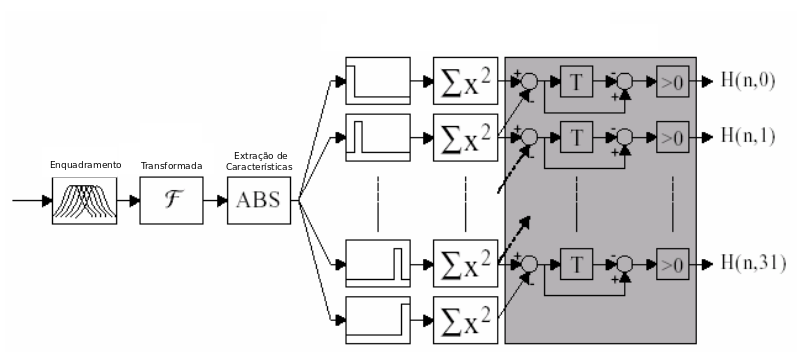
\includegraphics[scale=0.47]{figuras/extCaract.png}
   \\Fonte: \cite{haitsma2002}, adaptado pela autora
\end{figure}

A modelagem de \textit{fingerprint} geralmente recebe uma sequência de vetores de características calculadas quadro a quadro. As caracterísitcas escolhidas para montar o modelo de \textit{fingerprint} influenciam a forma como o algoritmo irá tratar futuramente a busca dessas características para comparação. Os modelos podem ser consultados em \cite{cano2005} e \cite{haitsma2002}. Uma forma compacta de \textit{fingerprint} é obtida, e assim, juntamente com informações sobre o formato de áudio original, é enviada para um servidor para identificação, como pode ser visto na Figura \ref{fig:identAudio}.

\begin{figure}[!htb]
   \centering
   \caption{Modelagem da identificação de áudio}\label{fig:identAudio} 
   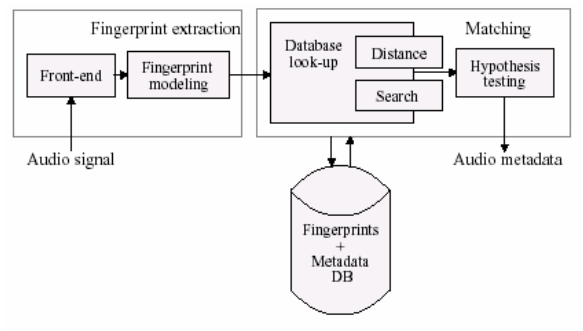
\includegraphics[scale=0.62]{figuras/etapasFinger2.png}
   \\Fonte: \cite{henriques2003}
\end{figure}

No segundo processo, denominado \textit{match}, há uma grande diversidade de algoritmos para localização, identificação e comparação de \textit{fingerprints}. Conforme mencionado anteriormente, o modelo de \textit{fingerprint} escolhido influencia a forma como o algoritmo irá à busca dessas características para comparação. Encontrar \textit{fingerprints} extraídas em um banco de dados de \textit{fingerprints} não é uma tarefa trivial. Em vez de procurar uma \textit{fingerprint} exata (fácil!), a \textit{fingerprint} mais semelhante precisa ser encontrada \cite{haitsma2002}.

A questão fundamental é como fazer a comparação eficiente do áudio desconhecido contra os possíveis milhões de \textit{fingerprints}. Uma abordagem de força bruta que calcule as semelhanças entre a \textit{fingerprint} da gravação desconhecida e as armazenadas no banco de dados pode ser proibitiva. O tempo para encontrar uma melhor correspondência é proporcional a \({N c(d()) + E}\), onde N é o número de \textit{fingerprints} no repositório e \({c(d())}\) o tempo necessário para uma única semelhança, sendo \({E}\) algum tempo extra da CPU \cite{cano2005}.

Alguns algoritmos citados por \citeonline{cano2005} são utilizados para medir a similaridade do conteúdo contido no modelo de \textit{fingerprint}:

\begin{itemize}
    \item K-\textit{Nearest Neighbors} ou K-NN, classificação do vizinho mais próximo usando uma estimativa de entropia cruzada.
    \item Distância Euclidiana, ou versões modificadas que lidam com sequências de diferentes comprimentos.
    \item Distância Manhattan, onde as sequências do vetor são quantizadas, ou distância Hamming quando a quantização é binária.
\end{itemize}

Esses algoritmos são descritos em mais detalhes nas subseções  \ref{subsubsec:classificacao} e \ref{subsubsec:medidas-similaridade}.

%===> CLASSIFICAÇÃO%
\subsubsection{Classificação} \label{subsubsec:classificacao}
Classificação é a tarefa de aprender uma função alvo \textbf{\({f}\)} que mapeie cada conjunto de atributos \textbf{\({x}\)} para um dos rótulos de classes \textbf{\({y}\)} pré-determinados \cite{pang2009}. A função alvo também é conhecida como modelo de classificação e, segundo \citeonline{pang2009}, pode ser classificada de duas formas:

\begin{itemize}
    \item Modelagem Descritiva: Pode servir como ferramenta explicativa para se distinguir entre objetos e classes diferentes. Por exemplo, explicar quais características definem uma música como Pop, Rock ou Jazz;
    
    \item Modelagem Preditiva: Pode ser usada para prever o rótulo da classe de registros não conhecidos, sendo tratada como uma caixa preta que atribui automaticamente um rótulo de classe quando recebe o conjunto de atributos de um registro desconhecido.
\end{itemize}

Técnicas de classificação são mais apropriadas para prever ou descrever conjuntos de dados com categorias nominais ou binárias, sendo menos efetivas para categorias ordinais.

Uma técnica de classificação é uma abordagem sistemática para construção de modelos de classificação a partir de conjuntos de dados de entrada. Cada técnica emprega um algoritmo de aprendizagem para identificar o modelo que seja mais apropriado para o relacionamento entre o conjunto de atributos e o rótulo de classe dos dados de entrada (Ver Algoritmo \ref{alg:classificacao}). O modelo gerado deve se adaptar bem aos dados de entrada e prever corretamente os rótulos de classes de registros que ele nunca viu antes \cite{pang2009}.

\begin{algorithm}[!htb]
    \SetAlgoLined
    Receber uma coleção de registros\;
    Encontrar um modelo  para determinar o valor do atributo classe em função dos valores de outros atributos\;
    Definir a classe de novos registros.
\caption{Algoritmo de Classificação básico}
\label{alg:classificacao}
\end{algorithm}

Os métodos de classificação podem ser divididos de duas formas: classificadores \textit{eager} (espertos) e classificadores \textit{lazy} (preguiçosos). Os classificadores espertos constróem um modelo de classificação capaz de classificar novos registros. Uma vez pronto o modelo, o conjunto de treinamento não é mais utilizado na classificação de novos registros. Exemplos de métodos que se enquadram nesta categoria são Árvores de Decisão, Redes Neurais, Redes Bayesianas e Naïve Bayes, Máquinas de Vetores de Suporte e Regras de Decisão.

Árvores de decisão são os classificadores espertos mais populares. Elas são representações gráficas que consistem em: (i) nodos que representam os rótulos das características (atributo); (ii) arcos que correspondem ao valor de uma característica e; (iii) nodos folha que representam uma classificação. Os métodos baseados em árvores, como o algoritmo ID3 (Ver Algoritmo \ref{alg:id3}), dividem o espaço de entrada em regiões disjuntas para construir uma fronteira de decisão. As regiões são escolhidas baseadas em uma otimização heurística onde a cada passo os algoritmos selecionam a variável que provê a melhor separação de classes de acordo com alguma função alvo \cite{vania2018-3}.
        
\begin{algorithm}[!htb]
    \SetAlgoLined
        Selecionar um atributo como sendo o nodo raiz\;
        Arcos são criados para todos os diferentes valores do atributo selecionado no passo 1\;
        Se todos os exemplos de treinamento (registros) sobre uma folha pertencerem a uma mesma classe, esta folha recebe o nome da classe. Se todas as folhas possuem uma classe, o algoritmo termina\;
        Senão, o nodo é determinado com um atributo que não ocorra no trajeto da raiz e arcos são criados para todos os valores. O algoritmo retorna ao passo 3.
    \caption{Algoritmo ID3 básico}
    \label{alg:id3}
    \end{algorithm}
    
    
No caso dos classificadores preguiçosos, cada novo registro é comparado com todo o conjunto de treinamento e é classificado segundo a classe do registro que é mais similar. Um exemplo de método bastante conhecido nesta categoria é o K-\textit{Nearest Neighbors}.
    
O K-\textit{Nearest Neighbors}, ou K-NN, é um classificador onde o aprendizado é baseado na analogia. O conjunto de treinamento é formado por vetores n-dimensionais e cada elemento deste conjunto representa um ponto no espaço n-dimensional.
    
Para determinar a classe de um elemento que não pertença ao conjunto de treinamento, o classificador procura K elementos do conjunto de treinamento que estejam mais próximos deste elemento desconhecido, ou seja, que tenham a menor distância. Estes K elementos são chamados de \textit{K-Nearest Neighbors} (K-vizinhos mais próximos). Verifica-se quais são as classes desses K vizinhos e a classe mais frequente será atribuída à classe do elemento desconhecido. O número de K-vizinhos é um parâmetro livre controlado pelo usuário com o objetivo de obter uma melhor classificação (ver Figura \ref{fig:knn}).
        
As métricas mais comuns utilizadas para o cálculo da distância são: Distância Euclidiana, Distância de Manhattan e Distância de Minkowski. Este processo de classificação pode ser computacionalmente exaustivo se considerado um conjunto com muitos dados, mas para determinadas aplicações, no entanto, o processo é bem aceitável \cite{knn2005}.
        
\begin{figure}[!htb]
     \centering
           \caption{K-Nearest Neighbors}\label{fig:knn} 
           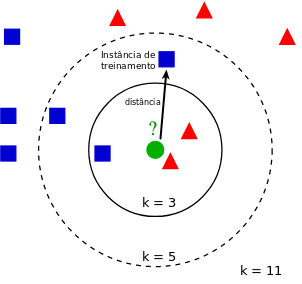
\includegraphics[scale=0.80]{figuras/knn.png}
           \\Fonte: Internet, adaptado pela autora
\end{figure}
        

%===> CLUSTERING%
\subsubsection{Clustering}\label{subsubsec:clustering}
A formação de agrupamentos (ou \textit{clustering}) divide os dados em grupos (\textit{clusters}) que tenham significado, sejam úteis, ou ambas as coisas. Se \textit{clusters} com significados forem o objetivo, então os \textit{clusters} devem capturar a estrutura natural dos dados.

O objetivo é que os objetos dentro de um \textit{cluster} sejam semelhantes (ou relacionados) entre si e diferentes de (ou não relacionados aos) objetos de outros \textit{clusters}. Quanto maior a semelhança (ou homegeneidade) dentro de um \textit{cluster} e maior a diferença entre \textit{clusters}, melhor ou mais distinto será o agrupamento \cite{pang2009}.

Encontrar o melhor agrupamento para um conjunto de objetos não é uma tarefa simples, a não ser que \textbf{\({n}\)} (número de objetos) e \textbf{\({k}\)} (número de \textit{clusters}) sejam extremamente pequenos, visto que o número de partições distintas em que podemos dividir \textbf{\({n}\)} objetos em \textbf{\({k}\)} \textit{clusters} é aproximadamente \textbf{\({k^n/k!}\)}, por exemplo, se \textbf{\({k=2}\)} e \textbf{\({n=5}\)} então são 16 formas de dividir 5 elementos em 2 \textit{clusters}.

A técnica de \textit{clustering} está relacionada a outras técnicas que são usadas para dividir objetos de dados em \textit{clusters}. Por exemplo, o \textit{clustering} pode ser considerado uma forma de classificação pelo fato de criar uma rotulagem de objetos com rótulos de classes (\textit{clusters}). Entretanto, ela deriva estes rótulos apenas dos dados \cite{pang2009}.

As principais abordagens de \textit{clustering} são as seguintes:

\begin{itemize}
    \item Particionamento (\textit{k-means} ou k-médias): é uma divisão do conjunto de objetos de dados, em um espaço \textbf{\({n}\)}-dimensional contínuo, em subconjuntos (\textit{clusters}) não interseccionados de modo que cada objeto de dado esteja exatamente em um subconjunto, ou seja, divide os dados em conjuntos disjuntos (\textit{clusters}) tal que cada ponto (objeto) pertence a um único cluster (ver Figura \ref{fig:kmeans}). É uma técnica particional de agrupamento baseada em protótipos que tenta encontrar um número especificado de \textit{clusters} (\textbf{\({K}\)}) pelo usuário, que são representados pelos seus centroides (ponto médio de um \textit{cluster} de pontos) \cite{pang2009}. A técnica de K-means é simples: Primeiro escolhe-se \textbf{\({K}\)} centróides iniciais e o número de \textit{clusters} desejado, que são parâmetros especificados pelo usuário. Cada ponto é atribuído a seguir ao centróide mais próximo, e cada coleção de pontos atribuídos a um centróide é um \textit{cluster}. O centróide de cada \textit{cluster} é então recalculado baseado nos pontos atribuído ao \textit{cluster}. Repete-se os passos de atribuição e recalculo até que os centróides permaneçam os mesmos. (Ver Algoritmo \ref{alg:kmeans} e aplicação do algoritmo na Figura \ref{fig:kmeansIteration}). O centróide é recalculado utilizando as medidas de similaridade e distância que podem ser vistas na subseção \ref{subsubsec:medidas-similaridade}.
    
    \begin{algorithm}[!htb]
        \SetAlgoLined
        Selecione K pontos como centróides iniciais\;
        \Repita{que os centróides não mudem}{
            Forme K clusters atribuindo cada ponto ao seu centróide mais próximo\;
            Recalcule o centróide de cada cluster\;
        }
    \caption{Algoritmo K-means básico}
    \label{alg:kmeans}
    \end{algorithm}
        
    \begin{figure}[!htb]
       \centering
       \caption{Usando o algoritmo K-means para encontrar três grupos nos dados de exemplo}\label{fig:kmeansIteration} 
       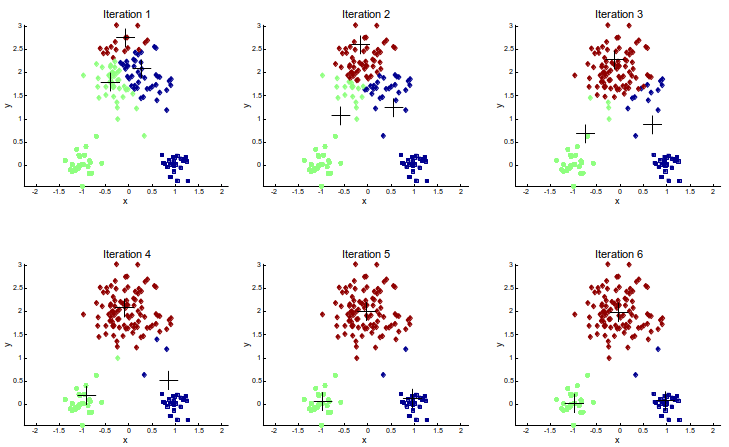
\includegraphics[scale=0.60]{figuras/iterationKmeans.png}
       \\Fonte: \cite{vania2018}
    \end{figure}
    
\begin{figure}[!htb]
       \centering
       \caption{Conjunto de objetos de dados em clusters}\label{fig:kmeans} 
       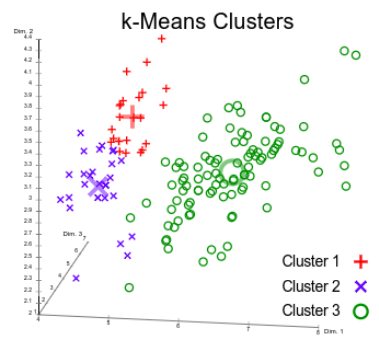
\includegraphics[scale=0.85]{figuras/kmeans.png}
       \\Fonte: \cite{kmeansCluster}
    \end{figure}    
    
    \item Hierárquico: se refere a um conjunto de técnicas de \textit{clustering} intimamente relacionadas que produzem um conjunto de \textit{clusters} aninhados organizados como uma árvore. Segundo \citeonline{pang2009}, há duas abordagens básicas para gerar um \textit{cluster} hierárquico:
    
    \begin{itemize}
        \item Aglomerativa: inicia com pontos individuais e, em cada etapa, funde os pares mais próximos em \textit{clusters}. Esta abordagem é expressa no Algoritmo \ref{alg:aglomerativo};
        
        \begin{algorithm}[!htb]
            \SetAlgoLined
            Calcule a matriz de proximidade, caso necessário\;
            \Repita{que reste apenas um \textit{cluster}}{
                Funda os dois \textit{clusters} mais próximos\;
                Atualize a matriz de proximidade para refletir a proximidade entre o novo \textit{cluster} e os \textit{clusters} originais\;
            }
        \caption{Algoritmo de agrupamento hierárquico aglomerativo básico}
        \label{alg:aglomerativo}
        \end{algorithm}
        
        \item Divisiva: inicia com um \textit{cluster} contendo todos os pontos e, a cada etapa, divide o \textit{cluster} até que restem apenas \textit{clusters} únicos de pontos individuais. Neste caso, precisamos decidir qual \textit{cluster} dividir em cada etapa e como fazer a divisão. Esta abordagem é expressa no Algoritmo \ref{alg:divisivo};
        
        \begin{algorithm}[!htb]
            \SetAlgoLined
            Calcule a matriz de distância, caso necessário\;
            \Repita{que restem apenas \textit{clusters} únicos}{
                Crie um novo \textit{cluster} para dividir o \textit{cluster} correspondente à maior diferença\;
            }
        \caption{Algoritmo de agrupamento hierárquico divisivo básico}
        \label{alg:divisivo}
        \end{algorithm}
        
    \end{itemize}
    
    Técnicas de agrupamento hierárquico aglomerativo são as de uso mais comum. A matriz de proximidade é o cálculo da similaridade entre dois \textit{clusters}. Ela é definida com um tipo específico de técnica de agrupamento hierárquico, como MIN, MAX e Média do grupo. MIN define a similaridade entre dois \textit{clusters} baseando-se nos dois pontos mais similares (mais próximos) dos dois clusters diferentes. De forma alternativa, MAX define a similaridade entre dois \textit{clusters} baseando-se nos dois pontos menos similares (mais distantes) entre dois \textit{clusters}. %(escolhe-se a menor distância máxima). 
    Já a Média do Grupo é dada pela média da distância entre pares de pontos nos dois clusters \cite{pang2009}. Uma técnica alternativa, o método de \textit{Ward}, supõe que um \textit{cluster} seja representado pelo seu centróide, mas mede a similaridade entre dois \textit{clusters} em termos do aumento do erro quadrado (similar à média do grupo, porém a distância entre os pontos é a distância ao quadrado) que resulta da fusão dos dois \textit{clusters}. Um cluster hirárquico é exibido frequentemente usando um diagrama do tipo árvore chamado dendograma, que exibe tanto os relacionamentos \textit{cluster}-sub\textit{cluster} quanto a ordem na qual os \textit{clusters} são fundidos ou divididos \cite{pang2009} (ver exemplo na Figura \ref{fig:dendograma}).
    
    \begin{figure}[!htb]
       \centering
       \caption{Um cluster hierárquico de quatro pontos mostrado como um dendograma e como grupos aninhados}\label{fig:dendograma} 
       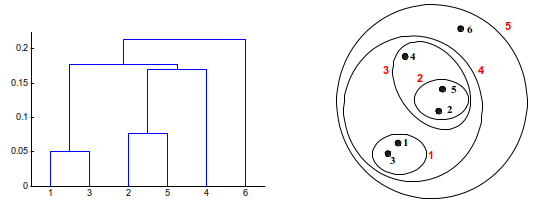
\includegraphics[scale=0.80]{figuras/dendograma.png}
       \\Fonte: \cite{vania2018-2}
    \end{figure}
    
    
    \item Baseadas em Densidade (DBSCAN): localizam regiões de alta densidade que estejam separadas entre si por regiões de baixa densidade \cite{ester1996}, sendo o algoritmo DBSCAN o principal representante desta categoria \cite{pang2009}.
    A densidade baseada em centro, seguida pelo DBSCAN, é avaliada para um determinado ponto no conjunto de dados contando-se o número de pontos dentro de um determinado raio (\textit{Eps}) a partir daquele ponto, que inclui ele próprio. Desta forma, é possível classificar um ponto como estando: \textit{(i)} no interior de uma região densa; \textit{(ii)} no limite de uma região densa; ou \textit{(iii)} em uma região ocupada esparsamente. Uma região densa é uma região onde cada ponto tem \textit{muitos} pontos em sua \textit{vizinhança} \cite{vania2018-2}. A vizinhança é determinada pelo raio Eps. Um ponto é central se o número de pontos dentro de uma determinada vizinhança têm pelo menos \textit{MinPts} (parâmetro especificado pelo usuário) em torno do ponto em questão. Um ponto de limite não é um ponto central, mas fica dentro da vizinhança de um ponto central. Um ponto de limite pode cair dentro das vizinhanças de diversos pontos centrais. Já um ponto ruído é qualquer ponto que não seja nem um ponto central nem um de limite \cite{pang2009}. Na Figura \ref{fig:dbscan}, o ponto 1 é um ponto central para o raio D (Eps) se MinPts \textbf{\({=}\)} 9. O ponto 2 é um ponto de limite e o ponto 3 é um ponto de ruído. O Algoritmo \ref{alg:dbscan} apresenta o DBSCAN. Quaisquer dois pontos de centro que estejam suficientemente próximos - dentro de uma distância Eps entre si - são colocados no mesmo \textit{cluster}. Da mesma forma, qualquer ponto de limite que esteja suficientemente próximo de um ponto de centro é colocado no mesmo \textit{cluster} do ponto de centro. Pontos de ruídos são descartados \cite{pang2009}. O DBSCAN pode lidar com \textit{clusters} de tamanhos e formas arbitrárias, conseguindo encontrar muitos \textit{clusters} que não podem ser encontrados utilizando o K-means.
   
    \begin{figure}[!htb]
       \centering
       \caption{Eps, pontos de centro, de limite e de ruído}\label{fig:dbscan} 
       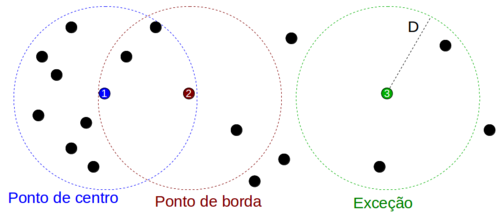
\includegraphics[scale=0.80]{figuras/dbscan.png}
       \\Fonte: \cite{wikilivros}
    \end{figure}
    
    \begin{algorithm}[!htb]
        \SetAlgoLined
        Rotular todos os pontos como de centro, de limite ou ruído\;
        Eliminar os pontos de ruído\;
        Colocar uma aresta entre todos os pontos de centro que estejam dentro da Eps uns dos outros\;
        Tornar cada \textit{cluster} de pontos de centro conectados a um \textit{cluster} separado\;
        Atribuir cada ponto de limite a um dos \textit{clusters} dos seus pontos de centro associados.
    \caption{Algoritmo DBSCAN}
    \label{alg:dbscan}
    \end{algorithm}
    
\end{itemize}

%===> CROSS RECURRENCE PLOT%
\subsubsection{Cross Recurrence Plot} \label{subsubsec:crossRecurrencePlot}
O trabalho de \citeonline{serra2009} propõe o uso de \textit{Cross Recurrence Plots} (CRP\abreviatura{CRP}{\textit{Cross Recurrence Plots}}) como métrica de similaridade entre músicas. Antes de definir CRP, é necessário introduzir o conceito de \textit{Recurrence Plot} (RP\abreviatura{RP}{\textit{Recurrence Plot}}). RP é uma ferramenta utilizada para visualizar recorrências com uma série temporal, ou seja, regiões onde a órbita da série passa perto de um estado previamente visitado. Mais especificamente, RP é uma matriz quadrada, preenchida com zeros e uns, que indica se há ou não recorrência, ou seja, se o estado no tempo \({i}\) é similar ao estado do tempo \({j}\) \cite{eckmann1987, alligood1996}. A diagonal principal de um RP é, portanto, composta por uns. CRPs são construídos da mesma maneira que RPs, mas cada eixo corresponde a uma série temporal diferente e a matriz resultante não é quadrada.

Primeiramente, o algoritmo extrai a característica HPCP \cite{gomez2006} de duas músicas, resultando em séries temporais de \({H = 12}\) variáveis. Dados os vetores HPCP da música \textbf{\({x}\)} e da música \textbf{\({y}\)}, calcula-se a transposição de \textbf{\({y}\)} de modo que ela fique na mesma tonalidade de \textbf{\({x}\)}. A transposição ocorre rotacionando-se o vetor HPCP de \textbf{\({y}\)} em \({k}\) posições por meio da técnica \textit{Optimal Transposition Index}, proposta em \cite{serra2009}.

A seguir, calcula-se o \textit{embedding} das duas músicas em um espaço de fase, isto é, um espaço onde as recorrências do sinal podem ser obtidas. Considere que  HPCP \textbf{\({x}\)} tem \({N_{x}^{*}}\) janelas. O \textit{embedding} de \textbf{\({x}\)} é dado por \({x' = \big\{x_{i}\big\}}\), para \({i = 1, ..., N_{x}, N_{x} = N_{x}^{*} - (m - 1)*\tau}\), em que \({x_{i}}\) é calculado conforme segue:
\begin{eqnarray} \label{embedding}
    x_{i} &=& (x_{1,i},x_{1,i+\tau}, \ldots, x_{1,i+(m-1)\tau}, \\
          & & x_{2,i},x_{2,i+\tau}, \ldots, x_{2,i+(m-1)\tau}, \nonumber \\
          & & \vdots \nonumber \\
          & & x_{H,i},x_{H,i+\tau}, \ldots, x_{H,i+(m-1)\tau}) \nonumber
\end{eqnarray}

Os autores estimaram os valores ótimos de \({m}\) e \({\tau}\) para o reconhecimento de músicas \textit{cover} por meio da divisão de uma base de dados em conjunto de treinamento e teste. Os parâmetros encontrados foram \({m = 10}\) e \({\tau = 1}\).

\citeonline{serra2009} utilizam a Equação \ref{crp} para calcular o CRP, em que \({\Theta(\cdot)}\) é a função degrau tipo Heaviside \({(\Theta(v) = 0 \ \textrm{se} \ v < 0 \  e \  \Theta(v) = 1, \ \textrm{caso contrário})}\), \({\epsilon_{i}^{x}}\) e \({\epsilon_{i}^{y}}\) são limiares de distâncias e \({|| \cdot ||}\) é a norma Euclidiana. No artigo, os autores calculam os limiares dinamicamente, de modo que 10\% dos vizinhos de cada entrada sejam considerados semelhantes.
\begin{equation} \label{crp}
    R_{i,j} = \Theta(\epsilon_{i}^{x} - ||\mathbf{x_{i} - y_{j}}||)\Theta(\epsilon_{i}^{y} - ||\mathbf{x_{i} - y_{j}}||)
\end{equation}

Em geral, pares de músicas diferentes não exibem nenhum padrão evidente no CRP e pares de músicas \textit{cover} apresentam estrutura de linhas longas e, caso contrário, tais padrões não ocorrem.

Com base no CRP de duas músicas, o trabalho de \citeonline{serra2009} propõe o uso do maior comprimento das diagonais formadas na matriz como métrica de similaridade. A medida \({Q_{max}}\) é definida como o maior comprimento das diagonais na matriz CRP, considerando possíveis variações no tempo da música (que correspondem a curvaturas nos traços) e na melodia (pequenas rupturas). Uma análise detalhada para o cálculo do \({Q_{max}}\) pode ser encontrada em \cite{serra2009}.

A partir da medida \({Q_{max}}\), é possível identificar grupos de músicas \textit{cover} em uma base de dados. Quanto maior o \({Q_{max}}\) entre duas instâncias, maior a probabilidade de elas serem interpretações diferentes da mesma música. Até hoje, \({Q_{max}}\) é considerado o estado da arte em métricas para identificação de músicas \textit{cover}. Sua principal desvantagem é seu alto custo computacional.

%===> DYNAMIC TIME WARPING%
\subsubsection{Dynamic Time Warping} \label{subsubsec:dtw}
O \textit{Dynamic Time Warping} (DTW\abreviatura{DTW}{\textit{Dynamic Time Warping}}) \cite{keogh2004} é uma técnica que permite definir uma métrica entre séries temporais, como por exemplo, características de áudio. Dadas duas séries \({Q}\) e \({C}\) de tamanhos \({n}\) e \({m}\), respectivamente, cria-se uma matriz \({D}\), \({n\times m}\), onde o elemento \({d_{i,j}}\) é a distância entre o elemento \({q_{i}}\) e \({c_{j}}\).

A partir da matriz \({D}\), o algoritmo procura por um caminho mínimo \({W}\), onde \({w_{k} = (i,j)_{k}}\), que respeite as seguintes condições:

\begin{itemize}
    \item Comece em \({(1,1)}\) e termine em \({(n,m)}\);
    \item Percorra apenas índices adjacentes;
    \item Percorra espaçamentos iguais no tempo.
\end{itemize}

O caminho mínimo é encontrado por meio de um algoritmo de programação dinâmica de complexidade \({O(nm)}\) \cite{keogh2004}. A métrica de dissimilaridade DTW é dada por:
\begin{equation}
    DTW(Q,C) = min\left\{\sqrt{\sum_{k=1}^{K} D[w_{k}]}\right\}
\end{equation}

em que \({K}\) é o tamanho do caminho e \({D[w_{k}]}\) é o valor da entrada \({(i,j)_{k}}\) na matriz \({D}\). A Figura \ref{fig:dtw} ilustra a execução do algoritmo DTW.

\begin{figure}[!htb]
   \centering
   \caption{Execução do algoritmo de DTW. (A) Séries C e Q. (B) Matriz de distâncias. (C) Alinhamento das duas séries com o caminho mínimo.}\label{fig:dtw} 
   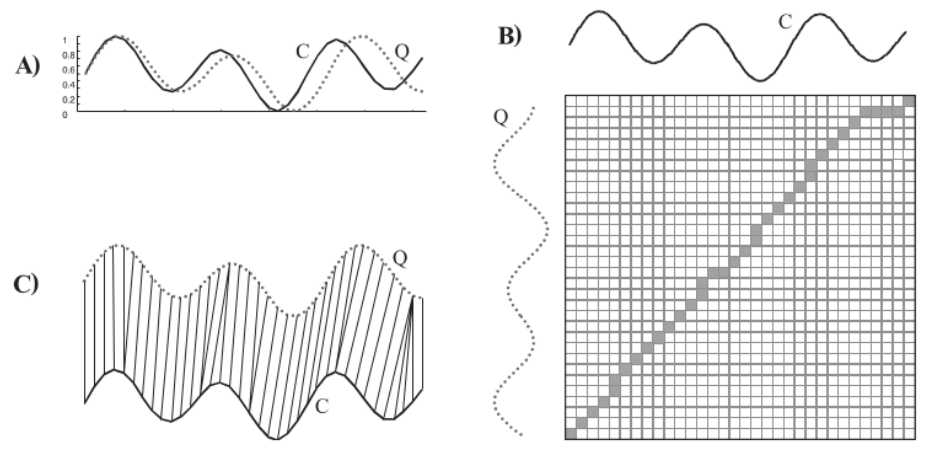
\includegraphics[scale=0.40]{figuras/dtw.png}
   \\Fonte: \cite{keogh2004}
\end{figure}

Seu uso é inviável em grandes conjuntos de dados. Por este motivo, diversas técnicas de indexação específicas para esse algoritmo foram propostas para a tarefa de busca por similaridade, tais como \textit{lower bound} e \textit{early abandoning}. Com essas técnicas, é possível encontrar os vizinhos mais próximos de uma dada subsequência em uma quantidade massiva de séries temporais. Informações mais detalhadas podem ser consultadas em \cite{mizutani2006}, \cite{kruskal1983} e \cite{juang1991}.

%===>>> RONALDO - 23/10/2018: ESTA SECAO ABAIXO DE INDEXACAO SE REFERE A ESTRUTURAS DE INDEXACAO ESPECIFICAS PARA DADOS MUSICAIS? DEIXAR CLARO ISSO NO INICIO DA SECAO 
%===>>> GISELE - 24/10/2018: O CONCEITO DE INDEXAÇÃO NÃO, MAS O EXEMPLO DETALHADO É ESPECIFICO PARA DADOS MUSICAIS.
%===>>> RONALDO - 30/10/2018: OK !

%===> INDEXAÇÃO%
\subsubsection{Indexação}\label{subsubsec:indexacao}
Estruturas de indexação (uma descrição sobre essas estruturas pode ser encontrada em [Garcia-Molina et al., 2002]) são normalmente fornecidas pelos SGBDs. A idéia básica dessas estruturas consiste na escolha de um objeto arbitrário central e na aplicação de uma função de distância para dividir os demais objetos em vários subconjuntos. Dessa maneira, uma estrutura de indexação é construída executando-se esse mesmo procedimento, recursivamente, para cada subconjunto não vazio \cite{barioni2006}.

Por exemplo, a \textit{Slim-tree} (um método aplicado à indexação de dados musicais) é uma árvore dinâmica e balanceada que cresce a partir das folhas em direção a raiz. Ela agrupa os objetos de um conjunto de dados em páginas de tamanho fixo, sendo que cada página corresponde a um nó da árvore. A \textit{Slim-tree} armazena todos os objetos nas folhas, organizando-os hierarquicamente na árvore. Essa hierarquia é construída a partir da seleção de objetos, denominados objetos representantes, que definem centros de regiões no espaço de dados. Cada região possui um raio de cobertura, e apenas os objetos que forem cobertos pelo raio de cobertura de uma determinada região podem ser armazenados nesse nó. Desta forma, cada nó da árvore
(exceto o nó raiz) possui, basicamente, um objeto representante, um raio de cobertura e os objetos do conjunto de dados que estão cobertos pela região do nó \cite{traina2000}.

Assim como a \textit{Slim-tree}, na literatura podem ser encontradas outros métodos aplicados à indexação de dados musicais, são a \textit{VP-tree} (\textit{Vantage Point tree}) \cite{yanilos1993}, a \textit{MVP-tree} (\textit{Multi-Vantage Point tree}) \cite{bozkaya1997}, a GNAT (\textit{Geometric Near-neighbor Access Tree}) \cite{brin1995}, a \textit{M-tree} \cite{ciaccia1997}, \textit{Família-Omni} e a \textit{DBM-tree} \cite{filho2001, vieira2004}, a \textit{n-grams} \cite{downie1999} e o \textit{Vantage Indexing Method} \cite{typke2003}.

%===> MEDIDAS DE SIMILARIDADE%
\subsubsection{Medidas de Similaridade} \label{subsubsec:medidas-similaridade}
A semelhança entre dois objetos é uma medida numérica do grau no qual os dois objetos se parecem. A diferença, ou dissimilaridade, entre dois objetos é uma medida númerica do grau no qual os dois objetos são diferentes. Frequentemente, o termo distância é usado como sinônimo de diferença, embora, muitas vezes seja usado para se referir a uma classe especial de diferenças.

Similaridade e distância são importantes pois são utilizadas por inúmeras técnicas de mineração de dados, como \textit{clustering} (ver subseção \ref{subsubsec:clustering}) e classificação (ver subseção \ref{subsubsec:classificacao}). Quanto menor o valor desta distância, mais semelhantes serão os objetos e eles tenderão a ficar no mesmo cluster. Quanto maior a distância, menos similares serão os objetos e, em consequência, eles deverão estar em grupos distintos.

Uma função de distância deve ser tal que:
\begin{itemize}
    \item Não assuma valores negativos (o menor valor é zero);
    \item Seja simétrica (a distância do objeto \textit{i} ao objeto \textit{j} deve ser a mesma distância do objeto \textit{j} ao \textit{i});
    \item Forneça o valor zero quando calculada a distância do objeto a si mesmo ou quando dois objetos são idênticos;
    \item Respeite a desigualdade triangular (dados 3 objetos, a distância entre dois deles tem que ser menor ou igual à soma das distâncias entre esses dois objetos e o terceiro).
\end{itemize}

Alguns algoritmos na literatura são utilizados para medir distância e similaridade:

\begin{itemize}
    \item Distância Euclidiana ou Distância Métrica: frequentemente utilizada com uma medida de distância entre dois pontos em planos n-dimensionais (ver Figura \ref{fig:euclidiana}), que pode ser provada pela aplicação repetida do teorema de Pitágoras. À medida que o número de dimensões aumenta, o tempo de cálculo também aumenta. A distância euclidiana entre os pontos \({P=(p_{1},p_{2},\ldots,p_{n})}\) e \({Q=(q_{1},q_{2},\ldots, q_{n})}\) num espaço euclidiano n-dimensional é expressa na Equação \ref{euclidiana}.
    
    \begin{equation} \label{euclidiana}
        \sqrt {(p_{1}-q_{1})^{2}+(p_{2}-q_{2})^{2}+\ldots +(p_{n}-q_{n})^{2}}=\sqrt {\sum _{i=1}^{n}(p_{i}-q_{i})^{2}}
    \end{equation}
    
    \begin{figure}[!htb]
       \centering
       \caption{Distância Euclidiana entre os pontos A e B}\label{fig:euclidiana} 
       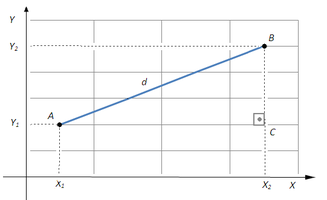
\includegraphics[scale=0.85]{figuras/euclidiana.png}
       \\Fonte: Internet
    \end{figure}
    
    \item Distância de Manhattan: medida de distância entre dois pontos em um espaço euclidiano com um sistema de cartesiano de coordenadas fixas (ver Figura \ref{fig:manhattan}). É a soma dos comprimentos da projeção da linha que une os pontos com os eixos das coordenadas. Em um plano que contém os pontos \({P_{1}}\) e \({P_{2}}\), com as coordenadas \({(x_{1},y_{1})}\) e \({(x_{2},y_{2})}\) respectivamente, essa distância é definida através da Equação \ref{manhattan}.
    
    \begin{equation} \label{manhattan}
        \left|x_{1}-x_{2}\right|+\left|y_{1}-y_{2}\right|
    \end{equation}
    
    \begin{figure}[!htb]
       \centering
       \caption{Distância de Manhattan (linhas roxa, verde e vermelha)}\label{fig:manhattan} 
       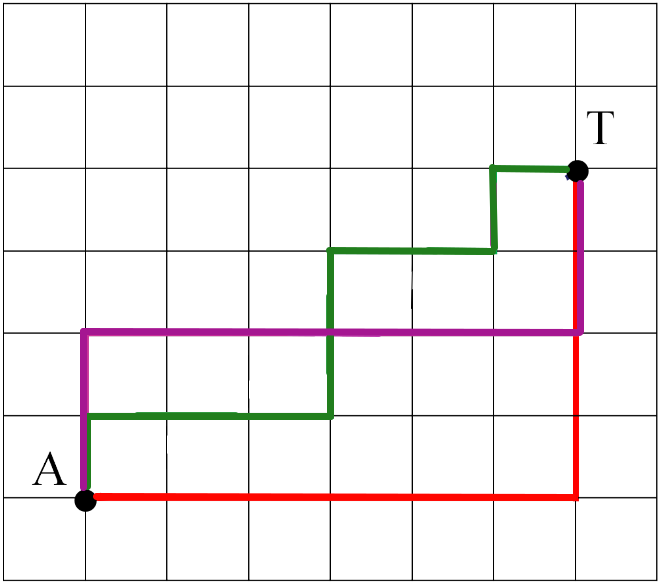
\includegraphics[scale=0.32]{figuras/manhattan.png}
       \\Fonte: Internet
    \end{figure}

    \item Distância de Minkowski: generalização das distâncias Euclidiana e de Manhattan (ver Figura \ref{fig:minkowski}), sendo definida pela Equação \ref{minkowski}. Quando \({q=1}\), esta distância representa a distância de Manhattan e quando \({q=2}\), a distância Euclidiana.
    
    \begin{equation} \label{minkowski}
        d(x,y)=(\left|x_{1}-y_{1}\right|_{q} + \left|x_{2}-y_{2}\right|_{q} + \cdots + \left|x_{n}-y_{n}\right|_{q})^{\frac{1}{q}}\textrm{, onde q} \in N
    \end{equation}
    
    \begin{figure}[!htb]
       \centering
       \caption{Distância de Manhattan (linhas rosa, verde e vermelha) e Distância Euclidiana (linha azul)}\label{fig:minkowski} 
       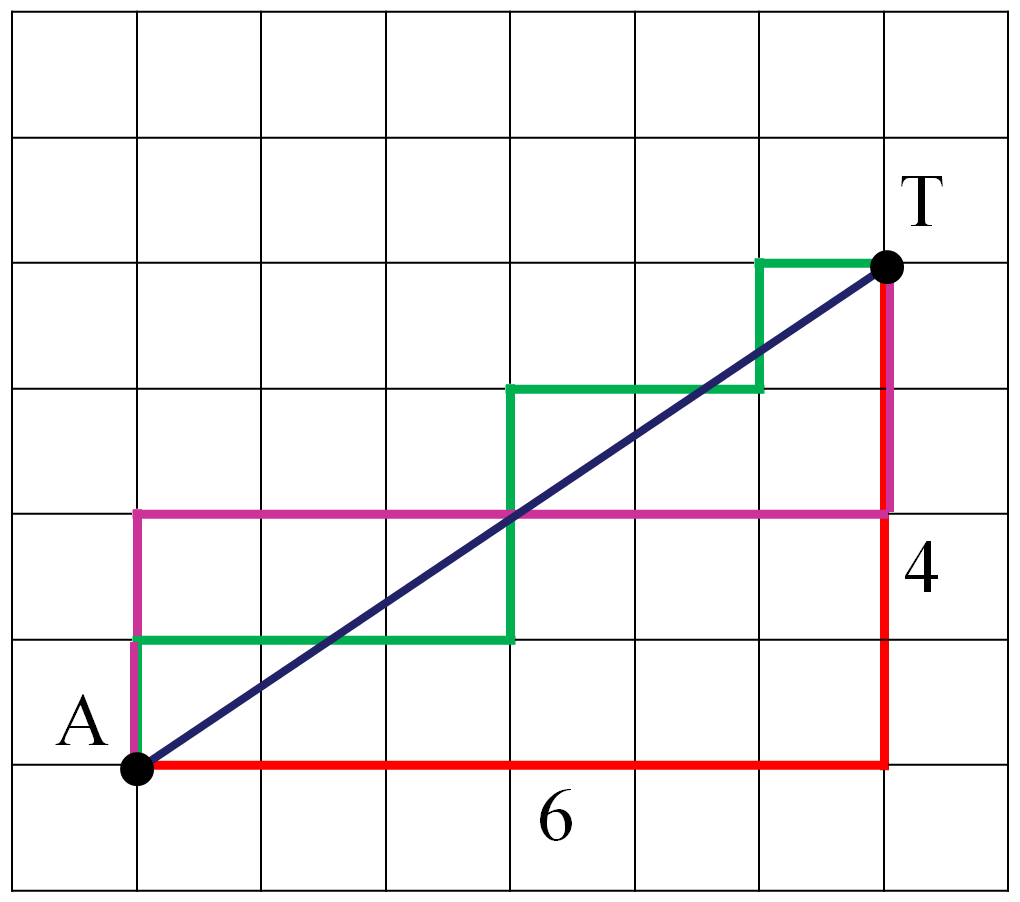
\includegraphics[scale=0.20]{figuras/minkowski.png}
       \\Fonte: Internet
    \end{figure}
    
    \item \textit{Longest Common Subsequence} (LCS): maior subsequência de caracteres comuns que há entre dois objetos (ver Figura \ref{fig:lcs}). Dadas duas sequências \({X}\) e \({Y}\) de comprimento \({m}\) e \({n}\), respectivamente, onde \({}\)
    \({X = \left\{X_{1}, X_{2}, \ldots, X_{m} \right\} }\) e \({Y=\left\{Y_{1}, Y_{2}, \ldots, Y_{n} \right\}}\) define-se \({LCS(X,Y)}\) como a máxima subsequência comum entre \({X}\) e \({Y}\). A equação de recorrência para o cálculo de \({LCS(X,Y)}\) pode ser deduzida a partir de duas propriedades:
    
    \begin{enumerate}
        \item Se \({X_{1}=Y_{1}}\), então \({LCS(X,Y)}\) é a concatenação de \({X_{1}}\) com \({LCS(X_{2:m},Y_{2:n})}\).
        \item Se \({X_{1} \not= Y_{1}}\), então \({LCS(X,Y)=max(LCS(X_{2:m},Y), LCS(X,Y_{2:n}))}\).
    \end{enumerate}

    Estas propriedades constituem a subestrutura ótima para a resolução continuada do primeiro caractere de cada string com a aplicação recursiva dessas mesmas propriedades ao sufixo remanescente. As mesmas propriedades são válidas quando as strings são analisadas do fim para o começo, resolvendo o último caractere e aplicando a recursão ao prefixo remanescente:
    
    \begin{enumerate}
        \item Se \({X_{m}=Y_{n}}\), então \({LCS(X,Y)}\) é a concatenação de \({LCS(X_{1:m-1},Y_{1:n-1})}\) com \({X_{m}}\).
        \item Se \({X_{m} \not= Y_{n}}\), então \({LCS(X,Y)=max(LCS(X_{1:m-1},Y), LCS(X,Y_{1:n-1}))}\).
    \end{enumerate}
    
    As definições matemáticas das recursões por sufixo e prefixo são respectivamente apresentadas nas Equações \ref{sufixo} e \ref{prefixo}.
    
    \begin{equation} \label{sufixo}
        LCS(X,Y) =
            \begin{cases}
            \emptyset & \quad \textrm{se } m=0 | n=0\\
            X_{1}+LCS(X_{2:m},Y_{2:n})  & \quad \textrm{se } X_{1}=Y_{1}\\
            max(LCS(X,Y_{2:n}),LCS(X_{2:m},Y)) & \quad \textrm{se } X_{1}\not=Y_{1}
            \end{cases}
    \end{equation}
    
    \begin{equation} \label{prefixo}
        LCS(X,Y) =
            \begin{cases}
            \emptyset & \quad \textrm{se } m=0 | n=0\\
            LCS(X_{1:m-1},Y_{1:n-1})+X_{m}  & \quad \textrm{se } X_{1}=Y_{1}\\
            max(LCS(X_{1:m-1},Y),LCS(X,Y_{1:n-1})) & \quad \textrm{se } X_{1}\not=Y_{1}
            \end{cases}
    \end{equation}
    
    \begin{figure}[!htb]
       \centering
       \caption{Longest Common Subsequence}\label{fig:lcs} 
       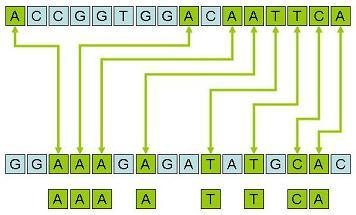
\includegraphics[scale=1.0]{figuras/lcs.jpg}
       \\Fonte: Internet
    \end{figure}
    
    Este algoritmo é apresentado com mais detalhes no trabalho dos autores \citeonline{cormen2009}.
\end{itemize}

Não há uma medida de similaridade que sirva para todos os tipos de variáveis que podem existir numa base de dados.

%===> QUERY BY HUMMING%
\subsubsection{Query by Humming} \label{subsubsec:qbh}
A tarefa de busca musical a partir de um trecho de música cantada ou cantarolada pelo usuário passou a ser conhecida na literatura como \textit{query by humming}, ou QBH. Trata-se de um sistema capaz de reconhecer música pelo \textit{casamento aproximado} de cadeias de caracteres. \citeonline{ghias1995}, autores do projeto, aplicaram o conceito de \textit{contorno melódico}, ou seja, a forma natural como nós percebemos a música. A Figura \ref{fig:qbh} mostra a arquitetura do sistema.

\begin{figure}[!htb]
   \centering
   \caption{Modelagem do Sistema de QBH}\label{fig:qbh} 
   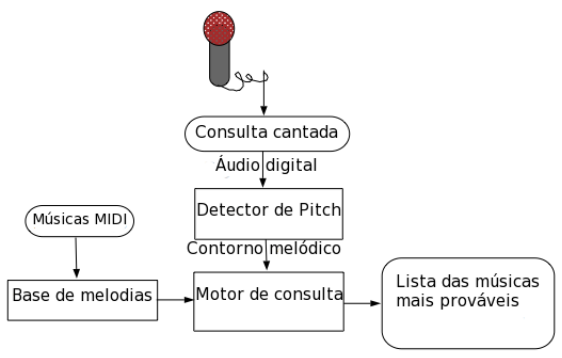
\includegraphics[scale=0.50]{figuras/qbh.png}
   \\Fonte: \cite{santos2011}
\end{figure}

Segundo \citeonline{santos2011}, existem dois principais interesses em QBH: Primeiramente, permitir ao usuário identificar uma música da qual não conheça (ou lembre de) qualquer metadado associado (autor, álbum, título da música, entre outros). Em segundo, é dispor de uma maneira mais natural para consultar coleções de músicas digitais armazenadas principalmente em dispositivos portáteis.

A base de dados de um sistema de QBH é, frequentemente, construída a partir da transposição de músicas MIDI para o formato de representação musical adotado pelo sistema (formatos vistos na seção \ref{sec:formatos}). Para casos em que a técnica de reconhecimento baseia-se em propriedades estatísticas associadas à incerteza do canto, é necessário também estimar os parâmetros do modelo. Para estimá-los, no entanto, precisamos de gravações da mesma música por diferentes usuários. Por este motivo, uma plataforma com este algoritmo estará em constante crescimento e aprendizado.

Capturar o sinal de áudio que codifica uma música cantada por um usuário, seja para construir a base de dados, seja para consultar o sistema por músicas conhecidas, requer atenção quanto ao nível de ruído do ambiente, à taxa de amostragem e à expressão fonética permitida. 

Conforme visto na subseção \ref{subsubsec:audioFingerprint}, alguns métodos utilizados no \textit{frontend} para a criação de uma \textit{fingerprint} também são utilizados para a segmentação e enquadramento do som utilizado pelo algoritmo QBH, deixando a representação musical em função do tempo.

Em seguida, a tarefa executada no sistema QBH é propor ao usuário uma lista de músicas que melhor correspondam à consulta, adotando uma medida de dissimilaridade apropriada entre os arquivos. A similaridade entre as músicas no repositório e a consulta é calculada por meio do DTW, visto na subseção \ref{subsubsec:dtw}, que o torna particularmente adequado para recuperação em sistemas QBH. O processo pode ser visto na Figura \ref{fig:qbhProcesso}.

\begin{figure}[!htb]
   \centering
   \caption{Sistema de QBH}\label{fig:qbhProcesso} 
   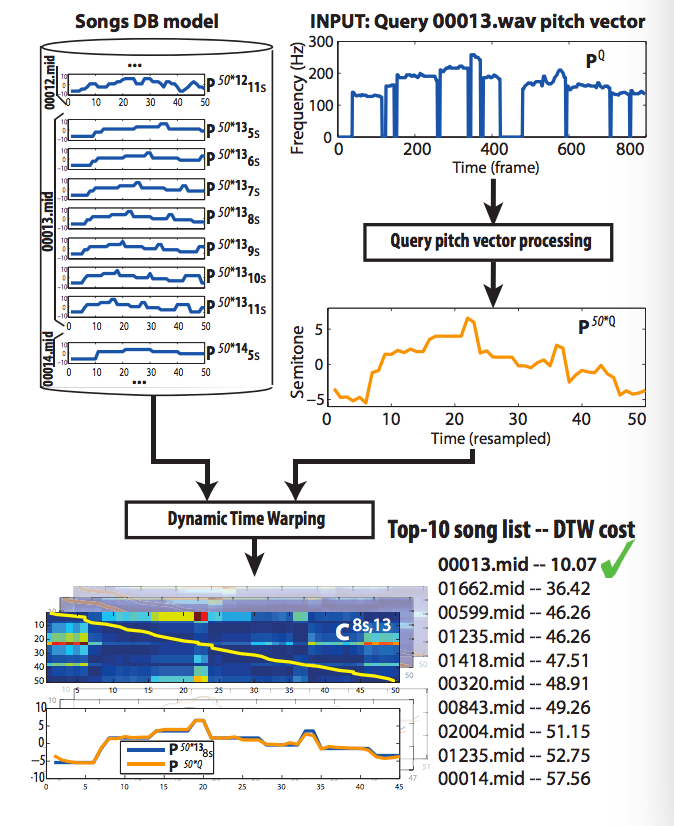
\includegraphics[scale=0.95]{figuras/query_by_humming.png}
   \\Fonte: ACRCloud
\end{figure}

Desta forma, vários tipos de sistemas QBH foram pesquisados:
\begin{itemize}
    \item \citeonline{wang2008} propuseram o sistema de QBH combinando as distâncias do \textit{earth mover’s distance} (EMD) e do \textit{dynamic time warping} (DTW) baseado na regra de soma ponderada.
    \item \citeonline{ryynanen2008} propuseram o método de extração dos vetores \textit{pitch} através do uso de uma janela de tempo de tamanho fixo e comparando-os por meio do método \textit{locality sensitive hashing} (LSH).
    \item \citeonline{salamon2009} propuseram recuperação em dois estágios para o sistema QBH. No primeiro estágio, o número de candidatos é reduzido através do método de indexação utilizando \textit{ngrams}. Depois, um método de comparação mais sofisticado é aplicado com os candidatos restantes baseado no alinhamento local com funções de custos modificados.
\end{itemize}

Embora os sistemas atuais de última geração para QBH tenham alcançado um desempenho razoável em casos do mundo real, ainda há muito espaço para a melhoria na indexação de músicas e o método de correspondência do sistema QBH, especialmente em um banco de dados de música na escala da Web.

%===> RECUPERAÇÃO POR CONTEÚDO%
\subsubsection{Recuperação por Conteúdo} \label{subsubsec:rpc}
A recuperação por conteúdo aplica-se a vários tipos de dados, inclusive música, e com o aumento da disponibilização de coleções de áudio digitais, se tornou importante permitir o gerenciamento automático desses tipos de dados por meio da utilização de metadados (ver seção \ref{sec:formatos}). Assim, várias técnicas de extração de metadados foram desenvolvidas, sendo algumas delas especialmente adequadas à recuperação de música por conteúdo.

As técnicas baseadas em busca por conteúdo utilizam metadados (como título, álbum e gênero da música) extraídos automaticamente dos dados musicais para representar e indexar as informações embutidas nos áudios digitais. O conjunto de metadados extraídos é chamado de \textit{vetor de características} \cite{tzanetakis2002}.

Nos sistemas de recuperação por conteúdo, as operações de comparação entre dados musicais utilizam os vetores de características para medir a similaridade do conteúdo presente nos dados que eles representam. Segundo \citeonline{barioni2006}, esse sistema possui quatro componentes principais:

\begin{itemize}
    \item Um módulo responsável pela extração automática de características que representem o conteúdo presente nos dados complexos;
    \item Um conjunto definido de métricas capazes de avaliar a similaridade entre os dados musicais;
    \item Uma interface de usuário que suporte tanto a definição dos parâmetros para a solicitação da consulta aos dados musicais quanto a visualização dos resultados obtidos;
    \item Um mecanismo de busca, que realiza as operações de busca sobre o conjunto de dados armazenados.
\end{itemize}

Várias áreas de pesquisa têm contribuído para o desenvolvimento de técnicas relacionadas a um ou mais dos componentes descritos acima. Dentre elas estão as técnicas para a extação automática de características de dados musicais; para a organização, indexação e consulta dos dados musicais; e para o gerenciamento de bases de dados musicais.

O módulo de extração de características é uma das bases fundamentais dos sistemas de recuperação de dados musicais por conteúdo. A sua importância está relacionada ao fato de que são as características extraídas por esse módulo que são utilizadas para a realização da indexação e da recuperação de dados musicais. O processo de extração de características consiste no cálculo de representações numéricas que podem ser utilizadas para caracterizar um determinado dado musical \cite{traina2003}.

Ao contrário das aplicações tradicionais de bases de dados que manipulam dados numéricos e textuais por meio da realização de consultas por igualdade e ordem, as aplicações que lidam com dados musicais requerem a realização de consultas por similaridade, ou seja, consultas que realizam busca por objetos da base que sejam similares a um objeto de consulta, de acordo com uma certa medida de similaridade. Para que um sistema de recuperação por conteúdo possa responder a consultas por similaridade, é necessário que ele seja capaz de mensurar o quão similar são os diferentes pares de objetos armazenados na base de dados bem como com o objeto de consulta, e é por meio da aplicação de métodos e algoritmos (ver subseção \ref{subsec:metodos-algoritmos-recuperacao}) que é obtida a quantificação dessa similaridade \cite{bohm2001, chavez2001}.

Porém, essa estratégia não é a mais adequada para ser utilizada em grandes conjuntos de dados, uma vez que o custo computacional envolvido é muito alto. Assim sendo, outro aspecto importante na recuperação de dados musicais por conteúdo está relacionado à utilização de estruturas de indexação (ver subseção \ref{subsubsec:indexacao}) apropriadas para espaços métricos que possam agilizar a realização de consultas por similaridade, ou seja, minimizar o número de cálculos de distância necessários para executar uma consulta.

%===> SPECTRAL MODELING SYNTHESIS%
\subsubsection{Spectral Modeling Synthesis} \label{subsubsec:sms}
\textit{Spectral Modeling Synthesis} (SMS\abreviatura{SMS}{Spectral Modeling Synthesis}), ou na sua tradução, Síntese de Modelagem Espectral, é uma abordagem de modelagem acústica para voz e outros sinais musicais. Ele considera os sons como uma combinação de conteúdo harmônico e conteúdo de ruído. Os componentes harmônicos são identificados com base em picos no espectro de freqüência do sinal, normalmente encontrados pela transformada de Fourier de curta duração (FFT). O sinal que permanece após a remoção dos componentes espectrais, por vezes referido como residual, é modelado como ruído branco passado através de um filtro que varia no tempo. A saída do modelo, então, são as frequências e níveis dos componentes harmônicos detectados e os coeficientes do filtro que variam no tempo.

\begin{figure}[!htb]
   \centering
   \caption{Análise de SMS e diagramas de bloco de síntese}\label{fig:smsProcesso} 
   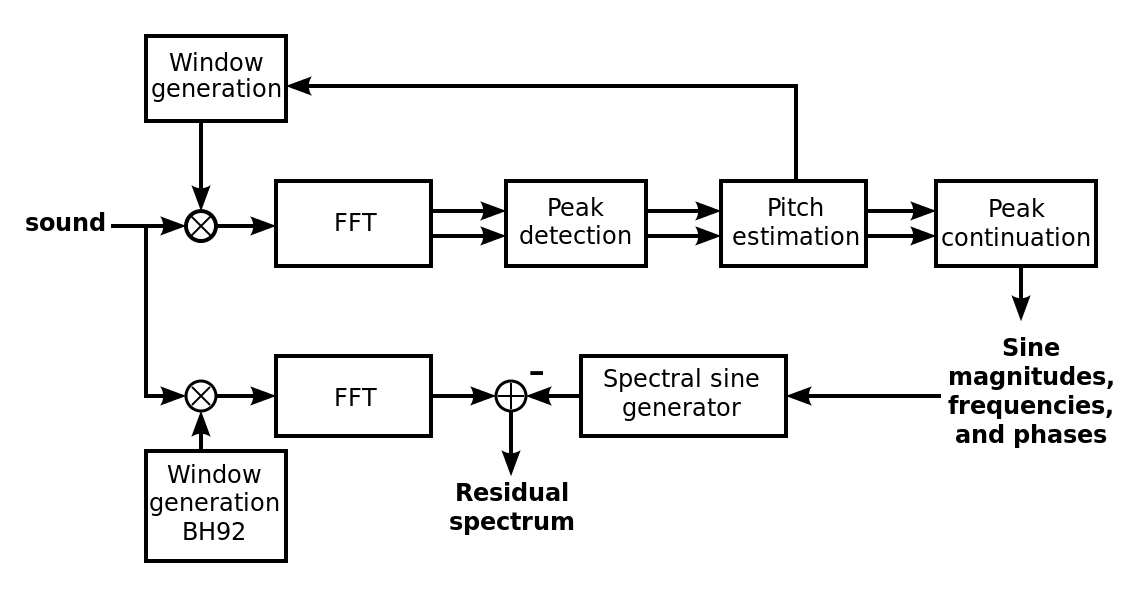
\includegraphics[scale=0.18]{figuras/sms.png}
   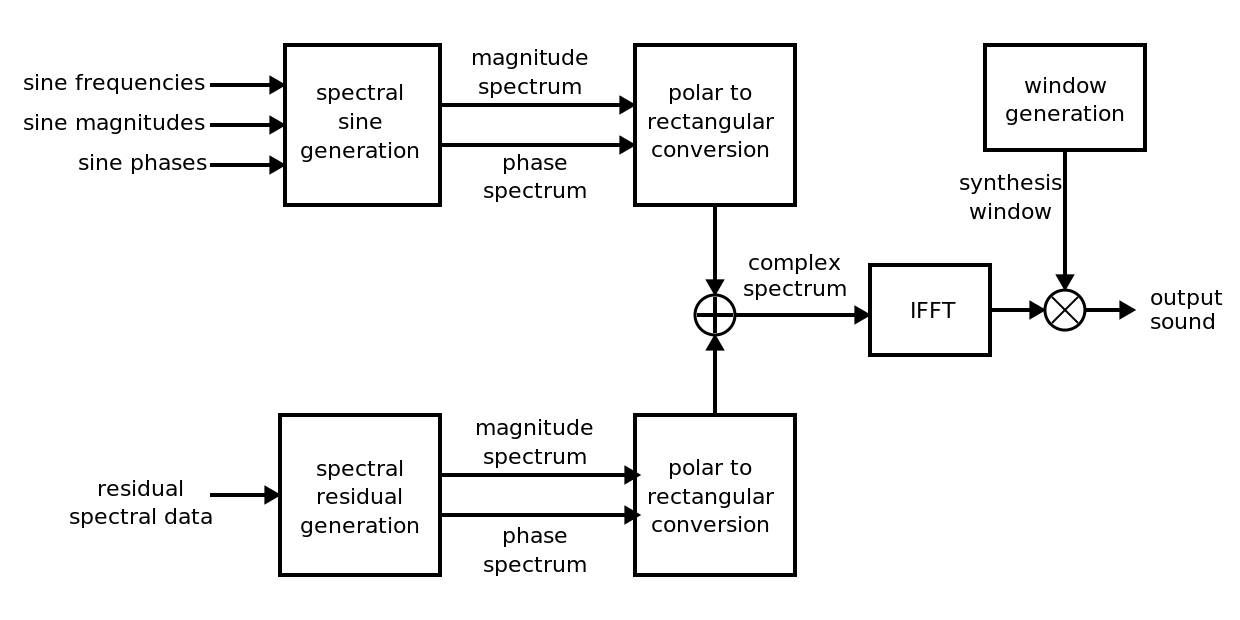
\includegraphics[scale=0.18]{figuras/sms2.png}
   \\Fonte: \cite{bonada2001}
\end{figure}

Na Figura \ref{fig:smsProcesso}, o procedimento de análise primeiro extrai as trajetórias senoidais rastreando os picos em uma sequência de FFTs. Esses picos são então removidos por subtração espectral. O $"$nível de ruído$"$ restante é modelado como ruído branco por meio de um filtro que varia no tempo. Uma aproximação linear por partes ao envelope espectral superior do ruído é calculada para cada espectro sucessivo, e a parte estocástica é sintetizada por meio da técnica de sobreposição-adição.

Intuitivamente, o modelo pode ser aplicado a muitos tipos de sinais de áudio. Os sinais de fala, por exemplo, incluem a mudança lenta dos sons harmônicos causados pela vibração das cordas vocais e sons de banda larga, semelhantes a ruídos, causados pelos lábios e pela boca. Os instrumentos musicais também produzem sons contendo componentes harmônicos e sons percussivos de ruído quando as notas são tocadas ou alteradas.

O modelo básico e a implementação foram desenvolvidos por \citeonline{serra1990}. Desde então, muitas extensões foram propostas, inclusive o SMS Tools, um conjunto de técnicas e implementações de software para análise, transformação e síntese de sons musicais baseados em várias abordagens de modelagem espectral. A técnica SMS provou fornecer transformações gerais de alta qualidade para uma ampla variedade de sinais musicais.

Essas técnicas podem ser usadas para aplicações de síntese, processamento e codificação, enquanto alguns dos resultados intermediários também podem ser aplicados a outros problemas relacionados à música, como separação de fontes sonoras, acústica musical, percepção musical ou análise de desempenho. Informações mais detalhadas sobre a técnica pode ser encontradas em \cite{serra1990}.

%===> VISUALIZAÇÃO%
\subsubsection{Visualização} \label{subsubsec:visualizacao}
Visualização de dados musicais é a exibição na forma de um gráfico ou tabela. Uma visualização bem sucedida requer que os dados sejam convertidos em um formato visual de modo que as carcterísticas dos mesmos e dos relacionamentos entre itens de dados possam ser analisados ou reportados. O objetivo da visualização é a interpretação da informação visualizada por uma pessoa e a formação de um modelo mental das informações \cite{pang2009}.

A principal motivação para o uso da visualização é que as pessoas podem absorver rapidamente grandes quantidades de informações visuais e encontrar padrões nas mesmas. Há diversas técnicas de visualização mencionadas na literatura. Este trabalho detalha a \textit{Self-Organizing Map} (SOM), em sua tradução, Mapas Auto-Organizados, que é utilizada por uma das soluções acadêmicas analisadas neste trabalho.

%===>>> RONALDO - 23/10/2018: NO PARAGRAFO ACIMA, POR QUE APENAS A TECNICA SOM EH DETALHADA? EH POR QUE ELA EH A MAIS APLICADA? OU ... (JUSTIFICAR)
%===>>> GISELE - 24/10/2018: POIS EXISTEM OUTRAS, ESOM É A TÉCNICA UTILIZADA POR UMA DAS SOLUÇÕES ACADÊMICAS, E É A DERIVAÇÃO DA TÉCNICA SOM, POR ISSO FALO APENAS DA TÉCNICA SOM.
%===>>> RONALDO - 30/10/2018: AUMENTEI O PARAGRAFO ACIMA PARA DEIXAR CLARO ISSO QUE TU RESPONDESTE ACIMA. TUDO OK AGORA.

A SOM é um tipo de rede neural artificial (ANN) que é treinada usando aprendizagem não supervisionada para produzir uma representação de baixa dimensionalidade (tipicamente bidimensional), chamado de mapa. Assim como em outros tipos de agrupamento baseado em centróides, como o K-means, o objetivo da SOM é encontrar um conjunto de centróides (vetores de referência) e atribuir cada objeto no conjunto de dados ao centróide que fornece a melhor aproximação desse objeto. Uma característica que distingue a SOM de outras abordagens de agrupamento é que ela impõe uma organização topográfica (espacial) pré-determinada sobre os centróides \cite{pang2009}. Em uma descrição de alto nível, a técnica SOM consiste dos passos descritos no Algoritmo \ref{alg:visualizacao}.

\begin{algorithm}[!htb]
    \SetAlgoLined
    Inicialize os centróides\;
    \Repita{que os centróides não mudem muito ou um limite seja atingido}{
    Selecione o próximo objeto\;
    Determine o centróide mais próximo do objeto\;
    Atualize este centróide e os centróides que estiverem próximos, i.e., em uma vizinhança especificada\;
    }
    Atribua cada objeto ao seu centróide mais próximo e retorne os centróides e grupos.
\caption{Algoritmo SOM básico}
\label{alg:visualizacao}
\end{algorithm}

%===>>> RONALDO - 23/10/2018: NO PARÁGRAFO ABAIXO, NAO ENTENDI A FRASE: "Uma SOM emergente difere de uma SOM tradicional em que um número muito grande de neurônios (pelo menos alguns milhares) é usado". QUAL EH A DIFERENCA AFINAL ??  
%===>>> GISELE - 24/10/2018: SOM É A REPRESENTAÇÃO DE BAIXA DIMENSIONALIDADE, SUA DERIVADA ESOM É PARA A REPRESENTAÇÃO DE ALTA DIMINSIONALIDADE. NO PARÁGRAFO DA LINHA 837 É DITO: "A SOM é um tipo de rede neural artificial (ANN) que é treinada usando aprendizagem não supervisionada para produzir uma representação de baixa dimensionalidade" E NO PARAGRÁFO ABAIXO: "Argumenta-se que seja especialmente útil para visualizar conjuntos de dados esparsos e de alta dimensão", POR ESTE MOTIVO SE DIFERE NO NÚMERO DE NEURÔNIOS UTILIZADOS, POIS SOM É UMA REDE NEURAL (QUE TEM NEURÔNIOS ARTIFICIAIS).
%===>>> RONALDO - 30/10/2018: OK !

Como derivação da SOM, há a Emergent SOM (ESOM\abreviatura{ESOM}{\textit{Emergent Self-Organizing Maps}}), um mapa topográfico de auto-organização emergente muito recente. Argumenta-se que seja especialmente útil para visualizar conjuntos de dados esparsos e de alta dimensão, produzindo uma visão intuitiva de sua estrutura. Uma SOM emergente difere de uma SOM tradicional em que um número muito grande de neurônios (pelo menos alguns milhares) é usado \cite{ultsch2005-2}. Diz-se que a preservação de topologia da projeção tradicional da SOM é de pouca utilidade quando se usa mapas pequenos: o desempenho de uma pequena SOM é quase idêntica ao de um K-means, com \textbf{\({k}\)} igual ao número de nós no mapa \cite{ultsch2005}. Uma vantagem adicional de uma ESOM é que ela pode ser treinada diretamente no conjunto de dados disponível sem primeiro ter que executar um procedimento de seleção de recursos \cite{ultsch2003}. Os mapas ESOM podem ser criados e utilizados para análise de dados por meio da ferramenta \textit{Databionics ESOM Public}\footnote{http://databionic-esom.sourceforge.net/ }. Esta ferramenta permite ao utilizador construir mapas ESOM planos e não vinculados (isto é, toroidais) \cite{ultsch2007}.

\begin{figure}[!htb]
   \centering
   \caption{Mapa topográfico com pequenos pontos para as músicas}\label{fig:mapaTopografico}
   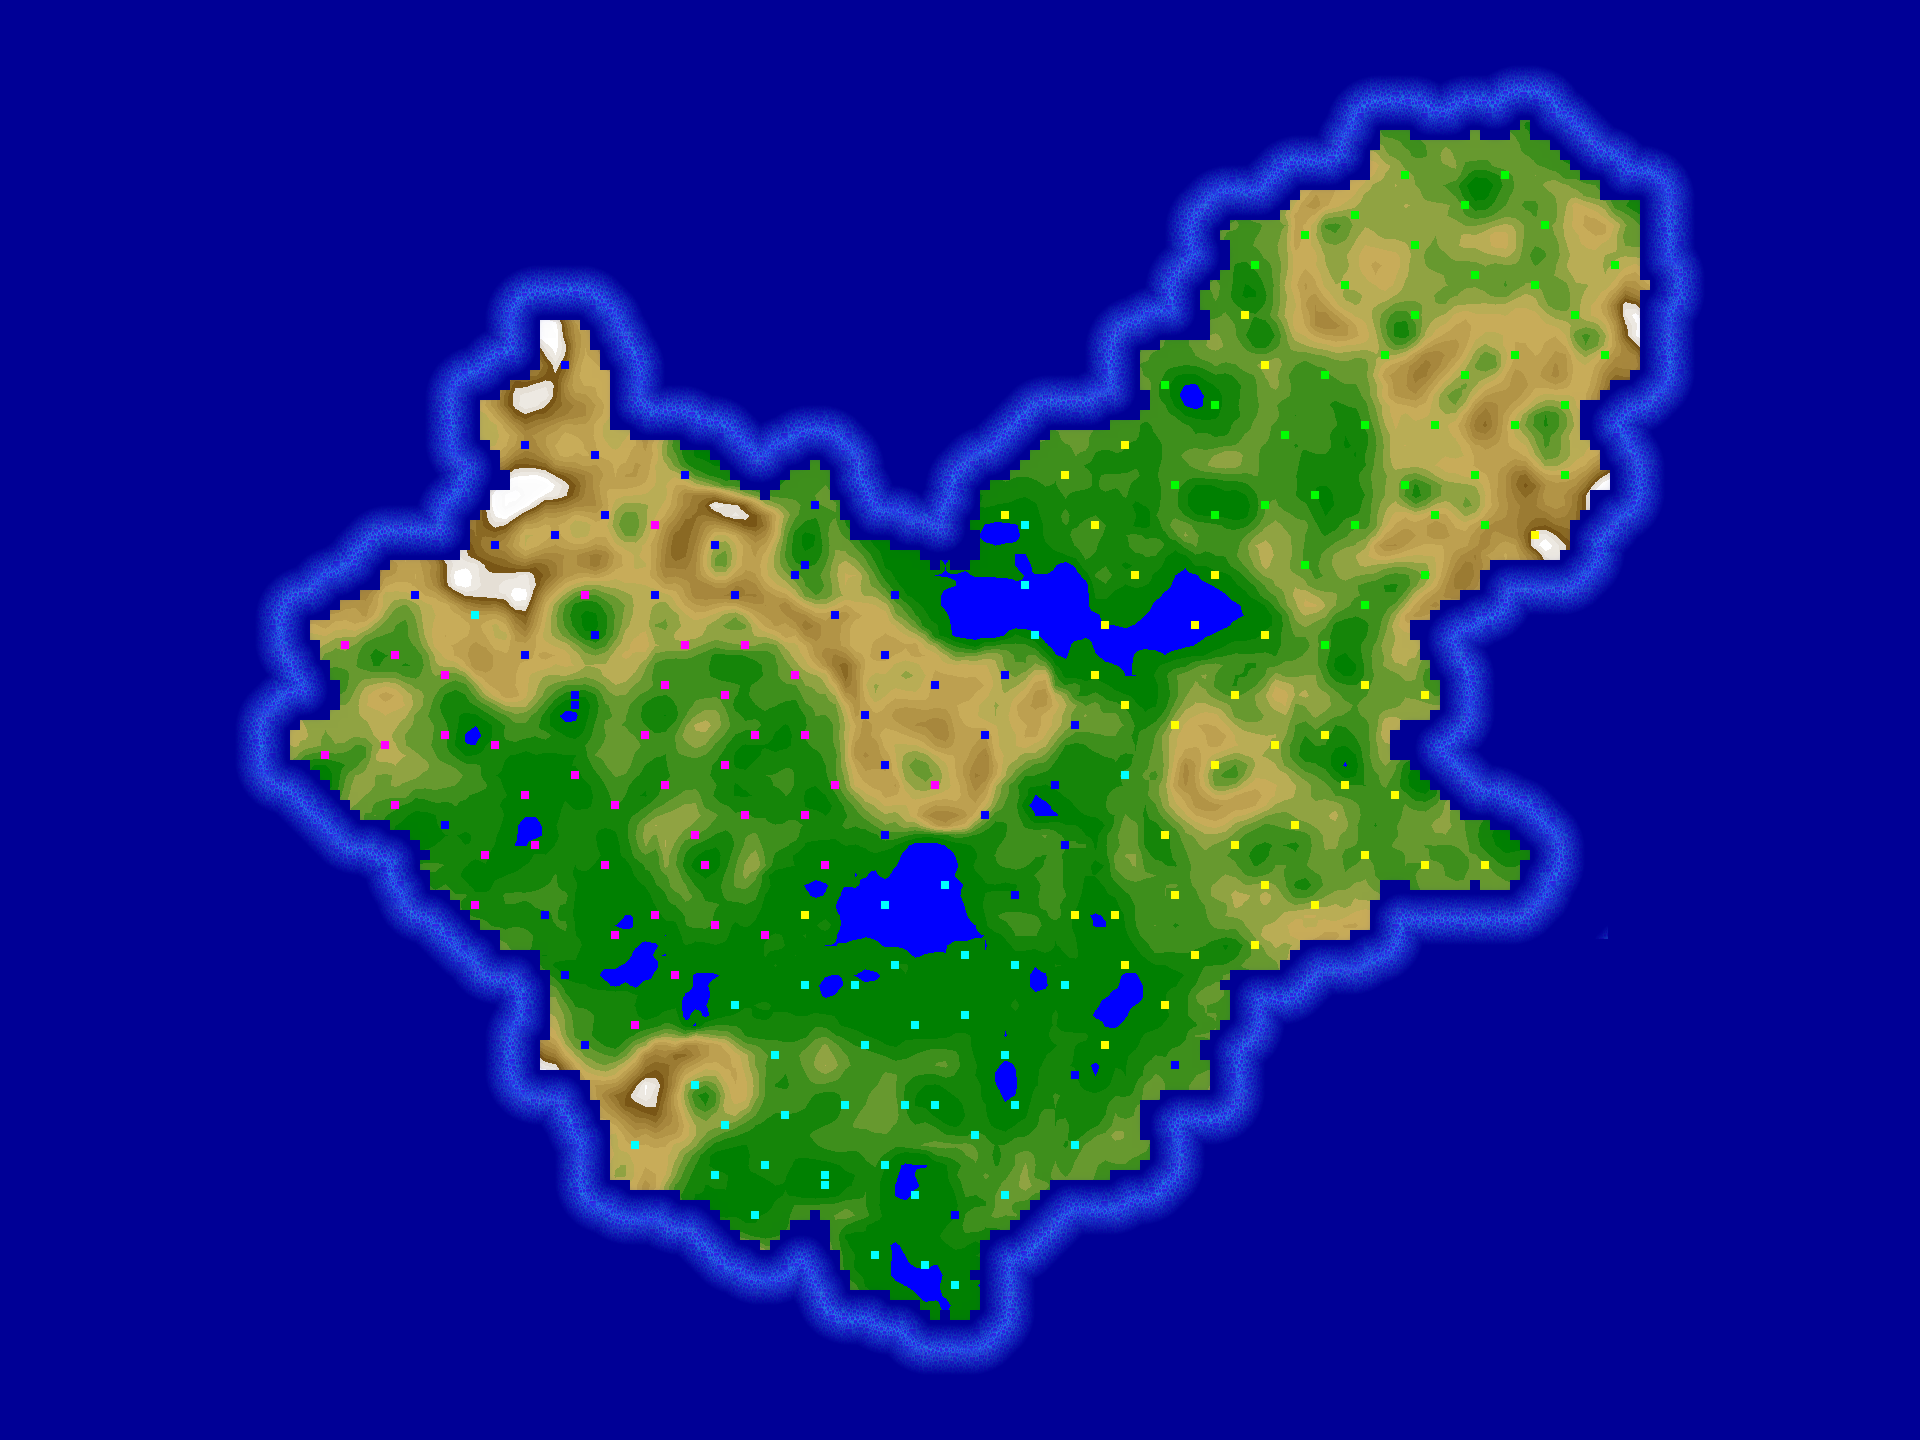
\includegraphics[scale=0.20]{figuras/musicmap.png}
   \\Fonte: \cite{musicminer}
\end{figure}

Na Figura \ref{fig:mapaTopografico}, é o resultado da aplicação da técnica ESOM, onde é possível visualizar a similaridade de músicas. De uma coleção de músicas, é extraído um mapa topográfico a partir de uma característica da música (por exemplo, gênero), e então, as sombras escuras e as bordas do mapa representam que os dados não possuem similaridade entre si. Já as sombras claras implicam na similaridade da respectiva característica extraída, ou seja, que há similaridade dos dados \cite{lohken2006}.

%===>>> RONALDO - 23/10/2018: A FIGURA ACIMA MOSTRA O QUE? O RESULTADO DA APLICACAO DA ESOM? DEIXAR MAIS CLARO. OUTRA COISA: NAO ENTENDI NADA DA FIGURA... SERIA BOM EXPLICA-LA MELHOR... 
%===>>> GISELE - 24/10/2018: AJUSTEI A EXPLICAÇÃO, VÊ SE FICOU MELHOR.